% Official IEEE template for IEEE Transactions on Dependable and Secure Computing
% (IEEE Template Selector: Computer_Society_LaTeX_template.zip, bare_jrnl_new_sample4.tex).
\documentclass[lettersize,journal]{IEEEtran}
\usepackage{cite}

\usepackage{amsmath,amssymb,amsfonts}
\usepackage{graphicx}
\usepackage{booktabs}
\providecommand{\multirow}[3]{#3}
\usepackage{array}
\usepackage{url}
\usepackage{algorithm}
\usepackage[noend]{algpseudocode}
\usepackage{hyperref}
\usepackage{xcolor}
\hypersetup{
  colorlinks=true,
  linkcolor=blue!60!black,
  citecolor=blue!60!black,
  urlcolor=blue!60!black
}

\renewcommand{\topfraction}{0.95}
\renewcommand{\bottomfraction}{0.95}
\renewcommand{\dbltopfraction}{0.95}
\renewcommand{\textfraction}{0.04}
\renewcommand{\floatpagefraction}{0.88}
\renewcommand{\dblfloatpagefraction}{0.88}
\setcounter{topnumber}{4}
\setcounter{bottomnumber}{4}
\setcounter{totalnumber}{6}
\setcounter{dbltopnumber}{4}

\newtheorem{property}{Property}
\newtheorem{lemma}{Lemma}
\algrenewcommand\algorithmicrequire{\textbf{Input:}}
\algrenewcommand\algorithmicensure{\textbf{Output:}}
\algrenewcommand\algorithmicindent{0.9em}
\begin{document}

\title{KEEPER: Defending Signed Trust Networks Against Erasure-Based Reputation Laundering}

\author{Muhammad~Usman and Yugyung~Lee%
\thanks{M. Usman and Y. Lee are with the School of Science and Engineering, University of Missouri-Kansas City (UMKC), Kansas City, MO, USA (e-mail: mucbp@umkc.edu; leeyu@umkc.edu).}%
\thanks{Corresponding author: Muhammad Usman.}%
\thanks{The code, configuration files, datasets, raw per-seed result files and a SHA-256 manifest (\texttt{MANIFEST\_SHA256.txt}) are available at \url{https://github.com/GreenPatterns/ReputationLaundering}. The repository's README maps each result to the files that produce it.}}

\markboth{IEEE Transactions on Dependable and Secure Computing}%
{Usman and Lee: KEEPER: Defending Against Erasure-Based Reputation Laundering}

\maketitle

\begin{abstract}
Graph neural networks can flag risky accounts from signed trust ratings, and privacy law lets raters erase them.
We show erasure can launder reputation: when a few raters delete authentic warnings about a distrusted account, the model stops ranking it as risky, although nothing was forged and unlearning was exact.
On four networks, deleting at most three warnings lifts targets on average from the platform's lowest 3\% to 7\% into its 25th to 34th percentile.
Removing the warnings from the frozen model's input reproduces the shift: the cause is missing evidence. The filters we tested pass most laundering requests.
KEEPER governs the evidence instead.
Its credibility layer provably bounds how many fake accounts one honest endorsement makes credible.
Against accounts exposed later, its escrow memory releases ratings gradually, letting credible warnings about their senders revoke the unreleased part.
Where lawful, its retention scheme keeps a deleted warning's verdict under a pseudonym of the rater's credibility tier, cutting the laundering gain by 98\% or more on three networks without accuracy loss relative to plain erasure.
Limits remain: escrow did not measurably change predictions, endorsed fakes still whitewash targets, insiders can link retained raters, and no preregistered statistical hypothesis survives multiplicity correction.
\end{abstract}

\begin{IEEEkeywords}
Signed trust networks, graph unlearning, reputation laundering, Sybil resistance, trust propagation, escrow memory, pseudonymous retention.
\end{IEEEkeywords}


\section{Introduction}
\label{sec:intro}

\IEEEPARstart{O}{nline} marketplaces, cryptocurrency exchanges and governance communities record who trusts whom.
Their signed trust networks store directed endorsements ($+1$) and warnings ($-1$) between accounts~\cite{kumar2016edge,kumar2018rev2,west2014exploiting}. Graph neural networks (GNNs) can learn which accounts are risky from these ratings~\cite{derr2018signed}, and dynamic GNNs re-score every account as new ratings arrive~\cite{rossi2020temporal}.
The same platforms are subject to data-protection law.
Article~17 of the General Data Protection Regulation (GDPR)~\cite{gdpr2016} gives users a conditional right to erase the ratings they wrote, and machine unlearning implements such erasure by removing the records and their influence from a trained model~\cite{cao2015towards,bourtoule2021machine,chen2022graph}.

This paper shows that the right to erasure opens a new way, which we call \emph{clean-data reputation laundering}, to rehabilitate a distrusted account (Fig.~\ref{fig:overview}a).
Suppose that an account $T$, the target, has received a few warnings and that their authors delete them, after an off-platform settlement, under pressure, or through ordinary churn.
Such pressure is documented: sellers on eBay pushed buyers to revoke negative feedback until the platform removed mutual feedback withdrawal~\cite{ye2014strategic}.
Every warning was authentic, every deletion is a legitimate request, and $T$ never changed.
Yet once the warnings are unlearned, the model no longer ranks $T$ among the accounts on which a platform would act.
On four signed networks, deleting at most three warnings raises the trust that a dynamic GNN predicts toward $T$, on average, by $0.347$ to $0.577$ on a scale from $0$ to $1$.
The targets move on average from their platform's lowest $3\%$ to $7\%$ into its $25$th to $34$th percentile.

\begin{figure*}[!t]
\centering
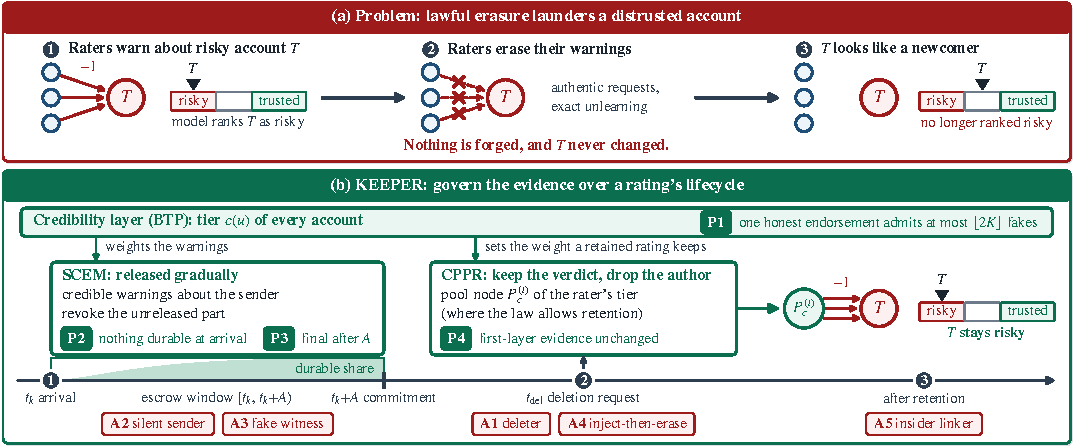
\includegraphics[width=\textwidth]{figures/fig_overview.pdf}
\caption{Clean-data reputation laundering and KEEPER. (a)~Raters lawfully erase their authentic warnings ($-1$) about a risky account $T$; after exact unlearning the model reads no trace of the warnings and no longer ranks $T$ as risky. (b)~KEEPER governs the lifecycle of a rating. An escrow memory (SCEM) releases the rating gradually until a commitment age $A$, while credible warnings about the rating's sender revoke the unreleased part. At deletion, a retention scheme (CPPR) keeps the rating's verdict under a pool node $P^{(t)}_c$, a pseudonym for the deleted raters of time window $t$ and credibility tier $c$. A credibility layer (BTP) supplies the tiers. Red tags mark where the five adversaries of Section~\ref{sec:threat_model} act, and green tags mark Properties~1 to~4 of Section~\ref{sec:keeper}.}
\label{fig:overview}
\end{figure*}

Laundering differs from the known attacks on unlearning and on graph models in three ways, and each difference disarms a family of defenses.
First, nothing is forged.
By contrast, poisoning attacks on unlearning plant crafted samples in the training data and later request their deletion~\cite{di2023hidden,zhang2026attack}, and graph attacks insert or remove edges of the adversary's choice~\cite{zugner2018adversarial}.
Mechanically, removing the warnings at a target is such a graph attack, restricted to deletions; what is new is the channel.
The ratings are removed by their own authors through requests that the platform normally honors. The attacker therefore needs no access to the graph, and every request that a filter inspects is authentic.
Second, the harm is the intended outcome of exact unlearning.
The closest attacks also leave the training data clean, but they select deletions so that the \emph{parameters} of the unlearned model misbehave on other inputs~\cite{zhao2023static,qian2023towards}.
In laundering, the deleted records are the evidence about the target itself, and the harmful model is the exact retrained model. A more accurate unlearning operator therefore cannot help.
Third, the effect comes from the graph that the model reads, not from its parameters: removing the warnings at inference, with every parameter frozen, reproduces $99.2\%$ to $100.3\%$ of the shift that full retraining causes.
Defenses that screen erasure requests or parameter updates therefore look in the wrong place.
The request filters that we tested pass $75.9\%$ to $100\%$ of the direct laundering requests, those that delete warnings about the target itself. Robust aggregation in federated training does not reduce the gain either.

A defense must instead govern the evidence itself.
If the platform must erase a warning and may retain nothing, no model can tell a laundered account from one that was never warned.
Where the law allows retention, the platform can keep the warning's verdict without its author.
Retained evidence, however, can be abused: fake accounts can rate a target and delete themselves so that retention keeps their ratings.
At the other end of a rating's lifecycle, on arrival, evidence also enters the model unchecked.
An account that is exposed only later can rate a target before any warning about that account exists, and a memory that commits on arrival makes the rating permanent.
A rating's weight is thus decided at two moments (Fig.~\ref{fig:overview}b): at \emph{commitment}, when the model's memory makes the rating permanent, and at \emph{deletion}, when its author withdraws it.

We present KEEPER (Keeping Evidence through Escrow and Pseudonymized Erased Ratings). It governs both moments with one quantity: the credibility of the account that supplies or contests a piece of evidence. KEEPER makes that credibility expensive for fake (Sybil) accounts to obtain.
Its \emph{credibility layer}, budgeted trust propagation (BTP), spreads a fixed budget of trust from early seed accounts along positive ratings and caps what each rating can carry.
One positive rating from an honest account then makes at most a fixed number of fake accounts credible, however many exist.
\emph{Source-Clocked Escrow Memory} (SCEM) governs commitment.
It releases each new rating into durable memory gradually and lets credible warnings about the rating's sender revoke the part not yet released. At a fixed commitment age, the rating's weight becomes final, which bounds the time in which an adversary can interfere.
Escrow could itself be abused by fake witnesses that warn about an honest rater to revoke that rater's warnings, so SCEM weights each witness by its credibility.
\emph{Credibility-Preserving Pseudonymous Retention} (CPPR) governs deletion where retention is lawful, for example for fraud prevention.
It keeps a deleted rating's verdict, that is, its target and its sign, but replaces the author by a pseudonym shared by all deleted raters of the same time window and credibility tier.
A deleted warning thus stays in what the model reads, and the rating of a fake account without honest endorsements keeps the lowest weight.
CPPR answers the deleter; SCEM does not act on the deleter and instead governs the other moment, commitment.

This paper makes three contributions.
\begin{enumerate}
  \item \textbf{A new threat.}
  To our knowledge, this is the first study of reputation laundering through the lawful erasure of authentic ratings.
  We measure laundering on four networks and trace it to the inference graph on all four, and for a second GNN on three of them. The request filters and robust aggregators that we tested do not stop it (Section~\ref{sec:laundering}).
  \item \textbf{KEEPER, three mechanisms with proved properties} (Section~\ref{sec:keeper}).
  The credibility layer makes at most $\lfloor 2Kg \rfloor$ fake accounts credible for $g$ honest endorsements, where $K$ is logarithmic in the number of accounts (Property~\ref{prop:btp}).
  The escrow memory makes nothing durable at arrival and bounds adversarial revocation in time and, for the witness evidence itself, in strength (Properties~\ref{prop:arrival} and~\ref{prop:window}).
  The retention scheme leaves a target's first-layer evidence unchanged, and every retained rating keeps its rater's tier weight (Property~\ref{prop:invariance}).
  \item \textbf{An evaluation under a protocol registered before the runs} (Section~\ref{sec:results}).
  On fresh training seeds, CPPR cuts the direct laundering gain by $98\%$ or more at no cost in accuracy relative to plain erasure.
  Credibility weighting reduces the share of an honest warning that fifty fake witnesses without honest endorsements revoke from escrow, on average, from between $16.5\%$ and $28.8\%$ to at most $0.34\%$, or $2.6\%$ if the fakes first build reliability by rating one another. The three registered exact checks hold.
  We report the limits with the same weight.
  None of the eight registered statistical hypotheses survives our correction for multiplicity; the effect of retention on direct laundering is large on all three networks and fails only the correction.
  Escrow did not measurably change predictions; a few fake accounts with an honest endorsement still whitewash a target; an insider can link retained raters; and in the combined system, ratings that pass through the escrow memory escape CPPR's credibility weighting.
\end{enumerate}
Section~\ref{sec:related} reviews related work, Section~\ref{sec:system} defines the setting and the threat model, Section~\ref{sec:laundering} studies the attack, Section~\ref{sec:keeper} presents KEEPER, Section~\ref{sec:results} evaluates it, and Section~\ref{sec:discussion} discusses its legal conditions and limitations.

\section{Related Work}
\label{sec:related}

This paper relates to three lines of work: unlearning and its attacks, Sybil-resistant reputation, and the memory and retention of evidence.

\smallskip\noindent\textbf{Unlearning and Its Attacks.}
Graph unlearning removes designated edges or nodes by retraining data shards~\cite{chen2022graph}, by first- or second-order parameter updates~\cite{wu2023gif,kurmanji2024towards}, or by only unlinking the deleted edges from the graph~\cite{tan2024unlink}; all of these treat full retraining as the benign ground truth.
Attacks on unlearning plant poison that deletion later activates~\cite{di2023hidden}; on graphs, they inject nodes whose requested deletion corrupts the unlearned model~\cite{zhang2026attack}. Other attacks exploit operators that erase more than requested~\cite{hu2024duty}, poison federated unlearning~\cite{unlearnguard2025}, or craft the deletion requests themselves on clean data~\cite{zhao2023static,qian2023towards}.
The last group is closest to our work. As Section~\ref{sec:intro} explains, these attacks make the parameters misbehave on other inputs, whereas in laundering exact retraining on the remaining evidence is itself the harm.
Our inject-then-erase adversary also injects accounts and deletes them, but it exploits retention, not an approximate unlearning operator.
Adversarial edits of a graph hurt more at the target than at its neighbors~\cite{zugner2018adversarial}, a finding that recurs in our comparison of direct and indirect deletion.
Byzantine-robust aggregators~\cite{blanchard2017machine,yin2018byzantine} filter abnormal parameter updates, which laundering does not produce.

\smallskip\noindent\textbf{Reputation and Sybil Defenses.}
Flow models such as EigenTrust~\cite{kamvar2003eigentrust} propagate positive trust, and signed models such as REV2~\cite{kumar2018rev2} and signed GNNs~\cite{derr2018signed} propagate both signs.
These models score the ratings that exist, whereas we study what happens when authentic ratings are withdrawn.
The classic way to shed a bad reputation is to re-enter under a new identity~\cite{friedman2001social}; laundering reaches the same end without one.
No reputation function that treats all accounts alike is Sybil-proof~\cite{cheng2005sybilproof}, which is why defenses start from trusted seeds~\cite{gyongyi2004combating}.
SybilGuard~\cite{yu2006sybilguard} and SybilRank~\cite{cao2012aiding} bound the influence of fake accounts with short random walks from such seeds, and SumUp~\cite{tran2009sybil} bounds bogus votes by the capacity of attack edges, the trust links from honest to fake accounts.
Our credibility layer adapts seeded propagation to directed endorsements.
Its bound has the order of SybilRank's, $O(\log n)$ fake accounts per attack edge, but it is a deterministic count that needs no assumption on how fast random walks mix; Section~\ref{subsec:results_btp} compares the two on our networks.
The layer also uses its output differently: its credibility tiers set the weight that a deleted but retained rating keeps, and the power that a witness holds over ratings in escrow.

\smallskip\noindent\textbf{Memory and Retention.}
Temporal Graph Networks~\cite{rossi2020temporal} write each event into memory on arrival and forget by decay.
SCEM instead delays permanence: its release follows the Erlang delays of gamma memories~\cite{devries1990gamma,hurtado2019generalized}, and evidence about the sender revokes what is not yet released.
Pseudonymization is a recognized safeguard for retained personal data~\cite{edpb2025pseudo}, yet the structure that remains around a pseudonym can re-identify an account~\cite{narayanan2009deanonymizing}. Our linkage test confirms such re-identification for retained ratings.

\section{Problem Setting}
\label{sec:system}

This section fixes the scoring model, the erasure operators, the adversaries and the design goals.
Table~\ref{tab:notation} lists the recurring notation; every other symbol is defined where it is used.

\begin{table}[!t]
\caption{Core notation.}
\label{tab:notation}
\centering
\footnotesize
\setlength{\tabcolsep}{3pt}
\begin{tabular}{@{}l>{\raggedright\arraybackslash}p{0.635\columnwidth}@{}}
\toprule
\textbf{Symbol} & \textbf{Meaning} \\
\midrule
$e_k = (u_k \to v_k, s_k, t_k)$ & rating $k$: sender, receiver, sign $\pm 1$, snapshot \\
$G_{\mathrm{train}}$, $F$ & training graph; forget set of deleted ratings \\
$r_\theta(v; G)$, $\Delta r$ & reputation of account $v$; laundering gain \\
$\mathcal{T}$, $T$ & cohort of distrust-majority accounts; a target \\
$\mathcal{U}_1$ to $\mathcal{U}_5$ & unlearning operators ($\mathcal{U}_1$ unlinks, $\mathcal{U}_2$ retrains) \\
$g$; $k$, $s$ & number of attack edges; numbers of fake witnesses and of fakes in a group \\
$q_i(v)$, $K$ & trust of $v$ after step $i$; number of propagation steps \\
$q_{\min}$, $q_{\mathrm{cap}}$ & trust threshold; cap per rating and step \\
$c(u)$, $w_c$ & credibility tier of $u$ in $\{0,1,2,3\}$; tier weight \\
$N$, $\phi$, $A$ & number of escrow stages, release rate, commitment age \\
$\lambda_u(t)$, $S_k(t)$ & hazard of sender $u$; survival of rating $k$ \\
$\omega_k$, $\pi_k$, $R_k$ & durable, escrowed and revoked mass of rating $k$ \\
$P^{(t)}_c$ & pool node of snapshot $t$ and tier $c$ \\
$\alpha^{(t)}_{u \to v}$ & credibility gate weight of a rating \\
\bottomrule
\end{tabular}
\end{table}

\subsection{Signed Trust Graph and Scoring Model}
\label{subsec:prelim}

A platform operator, the data controller, collects signed ratings, trains a scoring model on them, serves its predictions and processes erasure requests.

\smallskip\noindent\textbf{Graph.}
Let $G = (\mathcal{V}, \mathcal{E})$ be a directed signed multigraph of $n$ accounts whose edges are rating events.
A rating $e_k = (u_k \to v_k, s_k, t_k)$ records that sender $u_k$ rated account $v_k$ with sign $s_k \in \{-1, +1\}$ in snapshot $t_k$.
The ratings are cut in time order into $22$ snapshots (time windows) of nearly equal size; on Epinions-Dated (Table~\ref{tab:census}), the ratings that share the crawl timestamp form the first snapshot.
Models train on the first $21$ snapshots, which form the training graph $G_{\mathrm{train}}$ with edge set $\mathcal{E}_{\mathrm{train}}$; the last snapshot is held out for testing.
Account $v$ receives $d^+_{\mathrm{in}}(v)$ positive and $d^-_{\mathrm{in}}(v)$ negative ratings, and $\mathcal{E}^{(t)}_{\mathrm{in}}(v)$ is the set of ratings that $v$ receives in snapshot $t$.

\smallskip\noindent\textbf{Model.}
The backbone, LocalGDTE, is our dynamic signed GNN.
It starts from fixed diffusion features of $32$ dimensions, random vectors mixed with one diffusion step over the training graph. Three signed convolution layers then act within each snapshot. Each layer averages the representations of a node's neighbors and embeddings of the rating signs, separately over the ratings that the node issues and those that it receives.
Our temporal attention encoder, S3R, maps each account's sequence of snapshot embeddings to its final representation $z_v$. S3R is a causal sparse-attention block whose attention scores are biased by a selective state-space model~\cite{gu2023mamba}. A linear head maps the pair $[z_u \,\|\, z_v]$ to the probability $p_{uv}(G; \theta)$ that $u$ trusts $v$, where $\theta$ collects the trainable parameters.
A layer has no self term: it does not read the node's own representation. Every account without a rating in a snapshot therefore receives the same vector; Section~\ref{sec:laundering} repeats the attack with a self term.
Training minimizes the class-weighted cross-entropy of the training ratings (settings in Section~\ref{subsec:datasets}).

\smallskip\noindent\textbf{Reputation.}
The \emph{reputation} of an account $v$ estimates how likely ordinary accounts are to trust $v$: it is the predicted trust toward $v$, averaged over a fixed probe panel $\mathcal{P}$ of $256$ accounts drawn before any deletion,
\begin{equation}
\label{eq:canonical_rep}
r_\theta(v; G) = \frac{1}{|\mathcal{P} \setminus \{v\}|} \sum_{u \in \mathcal{P} \setminus \{v\}} p_{uv}(G; \theta).
\end{equation}
The reputation is derived from the model; it is not an observed enforcement log.
Most accounts have a high reputation, and a platform acts on the accounts that it ranks lowest, so we read reputations by rank. The \emph{platform percentile} of an account is the share of active accounts (those with at least one rating) whose reputation is lower.
As a working definition, the accounts on which a platform would act are the lowest tenth of this ranking.

\subsection{Erasure and Unlearning}
\label{subsec:operators}

When a forget set $F \subseteq \mathcal{E}_{\mathrm{train}}$ is deleted, the model reads the graph $G_{\mathrm{train}} \setminus F$, and an unlearning operator maps the trained parameters $\theta^\star$ to new parameters $\theta^{\mathrm{u}}$.
We evaluate five operators.
$\mathcal{U}_1$ (inference-only unlinking) keeps $\theta^\star$ and only removes $F$ from the graph that the model reads~\cite{tan2024unlink}.
$\mathcal{U}_2$ (full retraining) retrains from scratch on $G_{\mathrm{train}} \setminus F$ with the same seed and so produces the exact outcome that unlearning aims for.
$\mathcal{U}_3$ to $\mathcal{U}_5$ approximate retraining by updating $\theta^\star$: NegGrad+~\cite{kurmanji2024towards}, a damped Newton step on all parameters~\cite{wu2023gif}, and that step on the head alone.
Each operator shifts the reputation of an account $T$ by the \emph{laundering gain}, or gain for short,
\begin{equation}
\label{eq:gain}
\Delta r(T; F, \mathcal{U}) = r_{\theta^{\mathrm{u}}}(T; G_{\mathrm{train}} \setminus F) - r_{\theta^\star}(T; G_{\mathrm{train}}).
\end{equation}

\subsection{Threat Model}
\label{sec:threat_model}

The controller is trusted to train and serve the model on its own data and to run KEEPER as specified; raters and rated accounts are untrusted.
Table~\ref{tab:adversaries} lists the five adversaries by the stage of a rating's lifecycle at which they act.

\begin{table}[!t]
\caption{Adversaries, by the lifecycle stage at which they act (Fig.~\ref{fig:overview}b). Attack edge: a positive rating from an honest account to a fake one.}
\label{tab:adversaries}
\centering
\footnotesize
\setlength{\tabcolsep}{3pt}
\begin{tabular}{@{}l>{\raggedright\arraybackslash}p{0.19\columnwidth}>{\raggedright\arraybackslash}p{0.13\columnwidth}>{\raggedright\arraybackslash}p{0.53\columnwidth}@{}}
\toprule
 & \textbf{Adversary} & \textbf{Acts at} & \textbf{What it does} \\
\midrule
A1 & Deleter & deletion & Authentic raters erase their own warnings about a target, or their accounts; nothing is forged. \\
A2 & Silent sender & escrow & Rates a target and stays silent; warnings about the sender arrive only after a memory that commits on arrival has made the rating permanent. \\
A3 & Fake witness & escrow & $k$ fakes with $g$ attack edges warn about an honest rater to revoke that rater's warnings in escrow. \\
A4 & Inject-then-erase & deletion & $s$ fakes with $g$ attack edges rate a target and delete themselves, so that retention keeps their ratings. \\
A5 & Insider linker & after retention & Knows the pools and the model and tries to link a retained rating to its rater. \\
\bottomrule
\end{tabular}
\end{table}

\smallskip\noindent\textbf{Targets.}
A laundering target $T$ is a distrust-majority account, with more negative than positive incoming ratings.
The cohort $\mathcal{T}$ holds every such account of $G_{\mathrm{train}}$ with at most three negative ratings, the accounts for which a few deletions suffice:
\begin{equation}
\label{eq:cohort}
\mathcal{T} = \{T \in \mathcal{V} : d^-_{\mathrm{in}}(T) > d^+_{\mathrm{in}}(T) \text{ and } 1 \le d^-_{\mathrm{in}}(T) \le 3\}.
\end{equation}

\smallskip\noindent\textbf{The Deleter (A1).}
A1 needs no knowledge of the model.
\emph{Direct deletion} removes all negative ratings that enter $T$, or the accounts of their raters. \emph{Indirect deletion} removes negative ratings that enter $T$'s neighbors but no rating of $T$ itself.
The deletions are the raters' own requests; a request by $T$ to erase what others wrote about it is a weaker legal case (Section~\ref{subsec:gdpr}).

\smallskip\noindent\textbf{Fake Accounts and Attack Edges (A3, A4).}
Fake accounts are free to create, and they may rate anyone and one another.
What they cannot create is a positive rating from an honest account; we call such a rating an \emph{attack edge} and write $g$ for the number of attack edges.
On a trading platform an attack edge costs one transaction that an honest account rates well, so it is cheap but not free, and it leaves a trace at an honest account.
Like earlier Sybil defenses~\cite{cao2012aiding,tran2009sybil}, we treat attack edges as the scarce resource and measure what one or two of them buy.
A \emph{witness} of an account is any account that rates it; a fake witness (A3) warns about an honest rater so that escrow revokes that rater's warnings.
In the \emph{whitewash} variant of A4, the fakes rate a distrusted target $+1$; in the \emph{bad-mouth} variant, they rate a well-reputed target $-1$.

\smallskip\noindent\textbf{Assumptions.}
For A1, the training data contain no crafted poison and every deleted rating is authentic.
We do not model mistaken or retaliatory warnings: every warning counts as evidence (Section~\ref{subsec:limitations}).
A rater contributes at most one rating per rated account and occasion, such as a transaction or an election, as on our networks.
The seed accounts of the credibility layer are honest, and the controller can calibrate the layer on a graph without the fake accounts. In our experiments, this graph is the rating stream before any fake account is injected; a deployed platform would calibrate on accounts that it has reason to regard as honest.

\subsection{Design Goals}
\label{subsec:design_goals}

Against these adversaries, KEEPER pursues four goals.
\begin{itemize}
  \item \emph{G1, Sybil-bounded credibility.} The number of fake accounts that gain credibility is bounded per attack edge, and fakes without attack edges change no honest account's credibility.
  \item \emph{G2, revocable commitment.} A new rating is not permanent at arrival, and credible warnings about its sender revoke the part not yet permanent. After a fixed age, nothing can change the rating's weight.
  \item \emph{G3, laundering-free retention.} Under a lawful basis, a deleted rating keeps its verdict and exactly its rater's credibility weight, so deletion launders no target and upgrades no fake.
  \item \emph{G4, pseudonymous retention.} A retained rating carries no rater identity in the retained graph.
\end{itemize}

\section{Clean-Data Reputation Laundering}
\label{sec:laundering}

Before designing a defense, we measure the attack and locate its cause.
The study runs the deleter A1 against the backbone on four networks, and Fig.~\ref{fig:laundering} shows the main results.

\begin{table}[!t]
\caption{Signed networks and their laundering cohorts. Endorsed: cohort accounts with at least one endorsement. Edgeless: cohort accounts left without any rating after direct deletion. $^{\ast}$From the crawl date, the timestamp of $69\%$ of the ratings, to the last rating.}
\label{tab:census}
\centering
\footnotesize
\setlength{\tabcolsep}{1.5pt}
\begin{tabular}{@{}lrrrrrr@{}}
\toprule
\textbf{Network} & \textbf{Accounts} & \textbf{Ratings} & \textbf{Days} & \textbf{Cohort} & \textbf{Endorsed} & \textbf{Edgeless} \\
\midrule
Bitcoin-Alpha~\cite{kumar2016edge} & 3,783 & 24,186 & 1,901 & 135 & 21\% & 60\% \\
Bitcoin-OTC~\cite{kumar2018rev2} & 5,881 & 35,592 & 1,903 & 398 & 21\% & 65\% \\
Wiki-RfA~\cite{west2014exploiting} & 10,707 & 170,425 & 3,323 & 155 & 15\% & 69\% \\
Epinions-Dated~\cite{massa2005controversial} & 131,828 & 840,799 & 944$^{\ast}$ & 12,949 & 7\% & 69\% \\
\bottomrule
\end{tabular}
\end{table}

\begin{figure*}[!t]
\centering
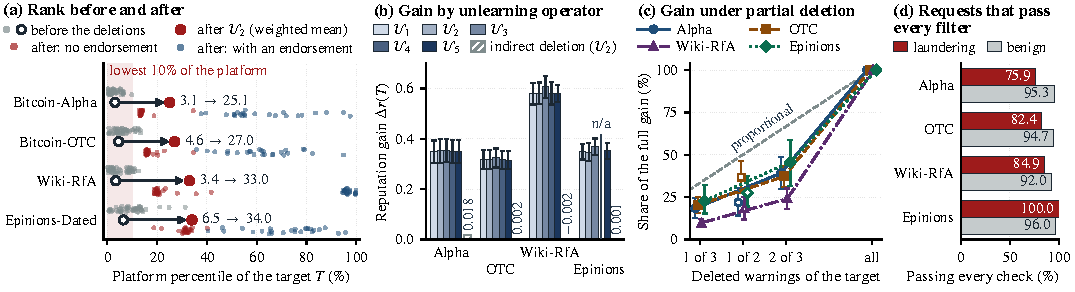
\includegraphics[width=\textwidth]{figures/fig_laundering.pdf}
\caption{Clean-data laundering on four networks (five seeds). (a)~Platform percentile of the targets before deletion and after exact retraining $\mathcal{U}_2$; large markers are cohort-weighted means, dots are targets, and the band is the lowest $10\%$ of the platform. (b)~Reputation gain of the sampled targets under the five unlearning operators and under indirect deletion (error bars: standard deviation across seeds; $\mathcal{U}_4$ was not run on Epinions-Dated). (c)~Share of the full gain under unlinking when only some of a target's warnings are deleted, with $95\%$ intervals (hollow: targets with two warnings). (d)~Erasure requests that pass every request-level check.}
\label{fig:laundering}
\end{figure*}

\smallskip\noindent\textbf{Setup.}
We use four signed networks (Table~\ref{tab:census}) and keep only the sign of each rating.
Bitcoin-Alpha and Bitcoin-OTC record trust between users of two Bitcoin trading platforms, Wiki-RfA records votes in Wikipedia administrator elections, and Epinions-Dated records trust in a review community.
The first three are fully dated and carry every experiment; Epinions-Dated is only partly dated and serves this study alone.
Triples of numbers always list Bitcoin-Alpha, Bitcoin-OTC and Wiki-RfA, followed by Epinions-Dated where it applies.
Per network, $50$ targets are drawn once from the cohort and attacked under five training seeds. On Bitcoin-Alpha and Wiki-RfA, two of these targets also serve to calibrate the approximate operators and are excluded, which leaves $48$.
The draw is stratified: $25$ targets come from the cohort accounts with at least one endorsement, or all of them when fewer exist, and the rest from the others. Endorsed accounts, only $7\%$ to $21\%$ of the cohort, are thus oversampled.
Cohort-level means therefore weight the two groups by their cohort shares, and we say so where we report them.
The study is exploratory, except for one hypothesis on the self term that we registered in advance (H8); Section~\ref{subsec:datasets} describes the protocol and the implementation.

\smallskip\noindent\textbf{Finding 1: Three Deletions Lift a Distrusted Account out of the Lowest Tenth.}
The sampled targets start from a mean reputation of $0.622$, $0.588$, $0.148$ and $0.454$. Because most accounts have a high reputation (Section~\ref{subsec:prelim}), the cohort nevertheless ranks on average in the lowest $3\%$ to $7\%$ of its platform.
Deleting at most three warnings about a target and retraining exactly raises its reputation by $+0.347$ to $+0.577$ in the cohort-weighted mean ($+0.317$ to $+0.581$ over the sampled targets).
On the platform's ranking, the cohort moves on average to between the $25$th and $34$th percentile, and $99.6\%$ to $100\%$ of the targets that start in the lowest tenth leave it (Fig.~\ref{fig:laundering}a).
The outcome has two modes.
Targets without an endorsement, $79\%$ to $93\%$ of the cohort, end at the $15$th to $31$st percentile, roughly a newcomer's score, and targets with an endorsement end between the $62$nd and the $97$th.
Deleting the raters' whole accounts gains about as much. On the three fully dated networks, targets with four or more warnings are laundered as well once all of their warnings are deleted ($+0.303$ to $+0.623$).
For scale, a placebo that deletes as many random ratings as warnings, all more than three hops from the target, moves its reputation by $0.018$ to $0.061$ on average under retraining.
The attack is hard to see in the model's utility: the mean change of the test Matthews correlation coefficient (MCC) lies between $-0.007$ and $+0.002$, and every $95\%$ interval includes zero.
Laundering also needs no coordination: when the $20$ most active negative raters leave a platform, $2.2\%$ to $10.2\%$ of the cohort rise, with frozen parameters, from below to above a reputation of $0.5$, the value at which the model predicts trust.

\smallskip\noindent\textbf{Finding 2: The Inference Graph Carries the Shift.}
Inference-only unlinking, which keeps every trained parameter, reproduces $99.2\%$ to $100.3\%$ of the gain of full retraining, and the approximate operators $\mathcal{U}_3$ to $\mathcal{U}_5$ also land close to the retraining gain (Fig.~\ref{fig:laundering}b).
The reason is a matter of scale. The deletion removes more than half of the ratings that $T$ ever received, yet less than $0.013\%$ of the training edges. It thus edits the graph around $T$ and leaves retraining almost nothing to adjust.
The finding is not specific to our backbone.
On the three fully dated networks, the Signed Graph Convolutional Network (SGCN)~\cite{derr2018signed}, a static GNN, gains $+0.355$ to $+0.603$ under the same deletions, and unlinking reproduces $97.8\%$ to $99.4\%$ of its retraining gain. EigenTrust~\cite{kamvar2003eigentrust}, in contrast, does not move: it propagates positive trust only, so it is neither laundered nor informed by the warnings.
A model that reads negative evidence is thus exposed through its input, not through its parameters.

The backbone also adds little beyond counting ratings.
Over the sampled targets, the gain is $1.29$ to $2.02$ times the shift of the Laplace-smoothed share of positive ratings that $T$ receives, $(d^+_{\mathrm{in}} + 1)/(d^+_{\mathrm{in}} + d^-_{\mathrm{in}} + 2)$. We do not read this factor as amplification learned by the model, for two reasons.
First, the factor falls to between $0.84$ and $1.44$ against a count that starts from the platform's base rate. Second, against the Laplace-smoothed share, the factor is concentrated in the targets left without ratings ($1.68$ to $2.22$, against $1.02$ to $1.89$ for the other targets).
Laundering is therefore a property of any score that reads negative evidence, not of the GNN.

The effect also follows the sign and the place of the erased evidence.
For the targets that hold endorsements, deleting an equal number of endorsements instead of the warnings and retraining lowers the reputation by $0.131$ to $0.265$.
Indirect deletion reaches at most $4.6\%$ of the direct gain over all targets, and $8.0\%$ over the targets for which indirect deletion is possible (Fig.~\ref{fig:laundering}b).
The reason is that each convolution layer averages over a node's ratings, once at the neighbor and again at $T$, which dilutes the deletion twice. Attacks through a target's neighbors are likewise the weaker ones in adversarial graph learning~\cite{zugner2018adversarial}.

\begin{figure*}[!t]
\centering
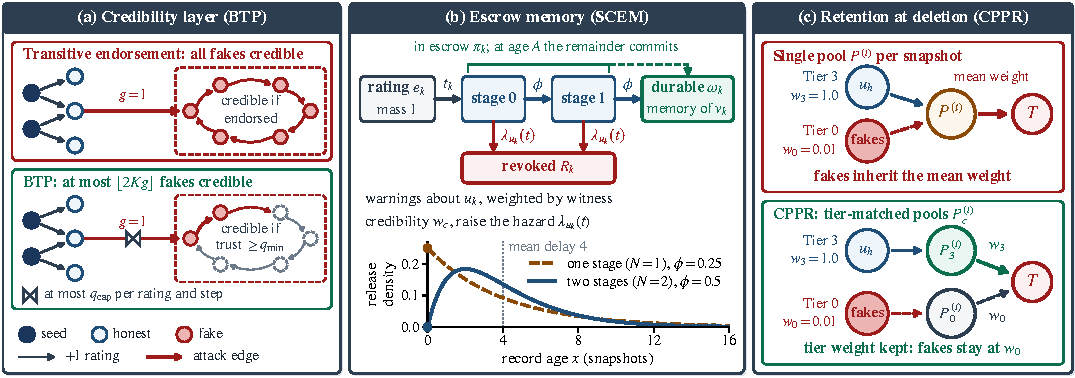
\includegraphics[width=\textwidth]{figures/fig_mechanisms.pdf}
\caption{KEEPER's mechanisms. (a)~Credibility layer: under transitive endorsement one attack edge makes a whole ring of fakes credible, whereas budgeted trust propagation carries at most $q_{\mathrm{cap}}$ per rating and step, so at most $\lfloor 2Kg \rfloor$ fakes reach $q_{\min}$. (b)~SCEM: the unit mass of a rating passes through two escrow stages into durable memory while the sender hazard $\lambda_{u_k}(t)$ revokes mass from both; the plot compares the release density of one and two stages at the same mean delay. (c)~CPPR: a single pool lets the ratings of Tier-$0$ fakes inherit the pooled raters' mean weight, whereas tier-matched pools keep every rating at its rater's tier weight.}
\label{fig:mechanisms}
\end{figure*}

\smallskip\noindent\textbf{Finding 3: The Last Warning Is Worth Most.}
Laundering is superadditive in the number of deleted warnings (Fig.~\ref{fig:laundering}c).
Under unlinking with fixed input features, deleting one of three warnings yields only $10\%$ to $23\%$ of the full gain, and deleting two of three yields $24\%$ to $46\%$.
The cause is a newcomer reset.
After the deletions, $60\%$ to $69\%$ of the cohort hold no rating at all, and the model gives all such accounts one score, that of an account it knows nothing about.
Under unlinking this score lies at the $14$th to $32$nd percentile, above the score of a warned account.
Most of the gain thus arrives with the deletion that removes the last warning. A partial collusion therefore buys little, and the evidence most worth protecting is a target's last remaining warning.
The reset persists when the backbone has a self term, although our registered criterion is met on one network only.
With a self term in every layer and fresh training seeds, unlinking still raises the targets' reputation by $+0.268$, $+0.340$ and $+0.435$ on the three fully dated networks, at a similar test MCC.
The registered criterion, at least half of the gain without a self term, is met on Wiki-RfA.
On the Bitcoin networks the intervals are wide and reach the criterion only at their upper end, so hypothesis H8 is not supported as registered.

\smallskip\noindent\textbf{Finding 4: The Filters We Tested Pass Most Laundering Requests, and Robust Aggregation Does Not Reduce the Gain.}
Checks of membership, role and rate pass every laundering request, because the requests are authentic.
A check on the direction of the unlearning update~\cite{unlearnguard2025} reacts most: it blocks $24.1\%$ of the direct laundering requests on Bitcoin-Alpha and none on Epinions-Dated.
In all, $75.9\%$ to $100\%$ of the direct requests pass every check, against $92.0\%$ to $96.0\%$ of benign requests (Fig.~\ref{fig:laundering}d).
Robust aggregation does not reduce the gain either.
In a federated variant on the Bitcoin networks, four clients hold contiguous blocks of snapshots, and the client that owns a target's warnings uploads its unlearning update.
The gain is measured there on the owning client's data after one aggregation round, so it is not comparable with the gains above.
Under plain averaging, the gain is $+0.7710$ and $+0.7097$. Under the coordinate-wise median, the trimmed mean, the geometric median and Krum~\cite{blanchard2017machine,yin2018byzantine}, it stays between $+0.7494$ and $+0.7712$ on Bitcoin-Alpha and between $+0.7100$ and $+0.7223$ on Bitcoin-OTC.
Even in the evaluations in which Krum returns a model without the unlearning update, the gain is still $+0.744$ and $+0.712$: the effect arrives through the graph that the model reads, not through an abnormal parameter update.

\smallskip\noindent\textbf{Implication: What a Defense Can Do.}
If the platform must erase a warning and may retain nothing, the served model depends only on a graph that holds no trace of the warning.
No model can then tell a laundered account from an account that never received the warning; when no rating remains, the latter is a genuine newcomer.
Suspicion toward newcomers, the classic answer to cheap identities~\cite{friedman2001social}, does not replace the missing evidence.
On the three fully dated networks, we shrink every reputation toward a cautious prior, the platform's $10$th percentile, with the weight of one extra rating.
In plain means over the sampled targets, the targets then end at the $24$th to $45$th percentile under unlinking instead of the $36$th to $57$th. Genuine newcomers, however, fall by $20$ to $42$ percentile points, and the test MCC on accounts with few ratings changes by $-0.109$, $+0.210$ and $-0.185$. A stronger prior makes the predictions for such accounts uninformative (MCC between $-0.02$ and $0.00$).
Against the deleter, a defense therefore has one opening: to retain the verdict of a deleted rating where the law allows it.
Retention in turn hands influence to whoever supplies ratings, so every piece of evidence must be weighted by a credibility that fake accounts cannot buy cheaply.
Beyond the deleter, a second route to an undeserved reputation needs no deletion at all: an account that is exposed only later rates a target before any warning about that account exists, and a memory that commits on arrival makes the rating permanent (adversary A2).
Evidence must therefore also stay revocable for some time after it arrives.
These three requirements (retention, credibility weighting and revocability) shape KEEPER.

\section{KEEPER}
\label{sec:keeper}

KEEPER governs a rating's weight at the two moments at which it is decided, commitment and deletion, with one quantity: the \emph{credibility} of the account that supplies or contests the evidence (Fig.~\ref{fig:overview}b).
A credibility layer assigns every account a tier that fake accounts cannot buy cheaply (Section~\ref{sec:btp}).
SCEM uses the tiers to decide whose warnings may revoke a rating in escrow (Section~\ref{sec:scem}), and CPPR uses them to weight retained ratings (Section~\ref{sec:cppr}).
Fig.~\ref{fig:mechanisms} illustrates the three mechanisms.

\subsection{Credibility Layer: Budgeted Trust Propagation}
\label{sec:btp}

\noindent\textbf{Intuition.}
An account is credible if accounts that are already credible endorse it.
The naive version of this rule, \emph{transitive endorsement}, starts from seed accounts and lets every positive rating from an endorsed account endorse its receiver.
Transitive endorsement fails against fake accounts: a single positive rating from an honest account admits a whole ring of fakes that endorse one another (Fig.~\ref{fig:mechanisms}a).
Budgeted trust propagation (BTP) instead derives credibility from trust, a conserved quantity.
Trust starts at early seed accounts and flows along positive ratings, and each rating carries at most a small, fixed amount per step. A group of fakes therefore receives trust only through its attack edges, and only a bounded amount per edge.

\smallskip\noindent\textbf{Propagation.}
Let the endorsement graph hold an edge $u \to v$ whenever the latest rating of $v$ by $u$ is positive, and let $d(u)$ be the number of accounts that $u$ endorses.
The seed set $\mathcal{S}_0$ holds the accounts with more positive than negative incoming ratings in the first five snapshots, and each seed $v$ starts with trust $q_0(v) = 1/|\mathcal{S}_0|$.
In each of $K$ steps, an account keeps half of its trust and offers the other half to its endorsees in equal parts, but one endorsement carries at most the cap $q_{\mathrm{cap}}$ per step:
\begin{equation}
\label{eq:btp}
\begin{aligned}
f_i(u \to v) &= \min\!\Big(\frac{q_i(u)}{2\,d(u)},\; q_{\mathrm{cap}}\Big), \\
q_{i+1}(v) &= q_i(v) - \sum_{v \to w} f_i(v \to w) + \sum_{u \to v} f_i(u \to v).
\end{aligned}
\end{equation}
The sender keeps whatever the cap withholds, so the total trust stays $1$.
The propagation stops early, after $K = \lceil \log_2 n_{\mathrm{ref}} \rceil$ steps for $n_{\mathrm{ref}}$ active accounts in the graph on which BTP is calibrated; stopping early keeps trust near the seeds, as in SybilRank~\cite{cao2012aiding}.

\begin{algorithm}[!t]
\caption{Budgeted trust propagation (credibility tiers)}
\label{alg:btp}
\footnotesize
\begin{algorithmic}[1]
\Require the ratings up to the snapshot of interest; frozen calibration $(\mathcal{S}_0, K, q_{\min})$
\Ensure tier $c(v) \in \{0, 1, 2, 3\}$ of every account $v$
\State build the endorsement graph and the counts $d(u)$
\State $q_0(v) \gets 1/|\mathcal{S}_0|$ if $v \in \mathcal{S}_0$, else $0$; \ $q_{\mathrm{cap}} \gets 2\,q_{\min}$
\For{$i = 0, \dots, K-1$}
  \State compute the capped flows $f_i$ and the trust $q_{i+1}$ by Eq.~\eqref{eq:btp}
\EndFor
\State trusted $\gets \{v : q_K(v) \ge q_{\min}\}$
\State eligible $\gets$ trusted accounts whose $+1$ ratings from trusted raters outnumber their $-1$ ratings from trusted raters
\State $c(v) \gets$ tercile ($1$, $2$ or $3$) of $q_K(v)$ among the eligible accounts if $v$ is eligible, else $0$
\end{algorithmic}
\end{algorithm}

\smallskip\noindent\textbf{Tiers.}
Algorithm~\ref{alg:btp} turns the final trust into tiers.
An account is \emph{trusted} if its trust reaches the threshold $q_{\min} = \varepsilon / n_{\mathrm{ref}}$, and the cap is $q_{\mathrm{cap}} = 2\,q_{\min}$.
The tolerance $\varepsilon$ is fixed on honest data.
The tolerance is the largest value of the registered grid $\{1, 0.5, 0.2, 0.1, 0.05\}$ at which BTP keeps at least $90\%$ of the accounts that transitive endorsement deems credible; when no value qualifies, the grid is extended by $\{0.02, 0.01, 0.005\}$.
The cap factor $2$ is the smallest of $\{1, 2, 4, 8\}$ for which this rule finds a qualifying $\varepsilon$ on all three networks; the factor was fixed after the probe of how many fakes one endorsement makes credible (Section~\ref{subsec:results_btp}) and before any trained attack run.
An account is \emph{eligible} if it is trusted and its positive ratings from trusted raters outnumber its negative ratings from trusted raters.
Eligible accounts receive Tiers~$1$ to~$3$ by the terciles of their trust, and every other account is in Tier~$0$.
Tier~$c$ carries the weight $w_c$, with $(w_0, w_1, w_2, w_3) = (0.01, 0.40, 0.70, 1.00)$.
We call an account \emph{credible} when its tier is $1$ or higher, and say that an endorsement \emph{admits} a fake account that becomes credible.
Counting only trusted raters in the eligibility test matters in both directions: the ratings of an untrusted account count neither for nor against anyone, so fakes without attack edges cannot lower the tier of an honest account.

\smallskip\noindent\textbf{Frozen Calibration.}
The seeds, the step count $K$ and the threshold $q_{\min}$ form the \emph{calibration}.
It is computed on the graph without the fake accounts and applied unchanged to the full graph, so fakes never become seeds and creating more fakes lowers no threshold.
CPPR computes the tiers once, on the training graph before any deletion.
SCEM needs a witness's tier at the time the witness rates. It therefore recomputes the tiers at every snapshot $t$ from the ratings before $t$, with one calibration per snapshot. We write $c_t(u)$ for this causal tier, which uses no future information.

\begin{property}[Bounded Sybil credibility, goal G1]
\label{prop:btp}
Let $\mathcal{B}$ be a set of accounts that holds no seed and receives $g$ attack edges, that is, endorsements $u \to b$ with $u \notin \mathcal{B}$ and $b \in \mathcal{B}$.
Under a frozen calibration, at most $\lfloor 2Kg \rfloor$ accounts of $\mathcal{B}$ are credible, whatever the size of $\mathcal{B}$, the ratings among its members and the trust of the endorsing accounts.
If $g = 0$, every account of $\mathcal{B}$ is in Tier~$0$, and every account outside $\mathcal{B}$ has the trust, the eligibility and the tier that it has in the graph without $\mathcal{B}$.
\end{property}
\begin{IEEEproof}
By Eq.~\eqref{eq:btp}, an account $v$ sends at most $d(v) \cdot q_i(v)/(2\,d(v)) = q_i(v)/2$, so trust stays non-negative. Every flow leaves one account and enters another, so trust is conserved.
Let $M_i = \sum_{b \in \mathcal{B}} q_i(b)$; $M_0 = 0$ because $\mathcal{B}$ holds no seed.
When Eq.~\eqref{eq:btp} is summed over $\mathcal{B}$, the flows between members cancel, the flows that leave $\mathcal{B}$ are non-negative, and the flows that enter $\mathcal{B}$ are those of the $g$ attack edges, each at most $q_{\mathrm{cap}}$.
Hence $M_K \le K g\, q_{\mathrm{cap}} = 2Kg\, q_{\min}$.
A trusted account holds at least $q_{\min}$, so at most $\lfloor 2Kg \rfloor$ accounts of $\mathcal{B}$ are trusted, and only a trusted account can be eligible.
For $g = 0$, $M_i = 0$ at every step, so no member holds trust or sends a flow.
No outside account endorses a member, so the counts $d(u)$ and, by induction over the steps, all flows outside $\mathcal{B}$ equal those in the graph without $\mathcal{B}$.
The eligibility test counts ratings from trusted raters only and the members are untrusted, so the eligible set, its tercile boundaries and every tier are unchanged.
\end{IEEEproof}

\smallskip\noindent\textbf{Remarks.}
The bound does not depend on the number of fakes or on how they rate one another. It does need the frozen calibration: if the calibration were recomputed on an attacked graph, each fake would raise $n_{\mathrm{ref}}$ and lower $q_{\min}$.
On our networks, $K$ is $12$, $13$ and $14$, so one attack edge makes at most $24$, $26$ and $28$ fakes credible, whereas transitive endorsement makes every fake credible.
With attack edges, the credible fakes join the eligible accounts and shift the tercile boundaries, so some honest accounts can change tier (Section~\ref{subsec:results_scem}).

\smallskip\noindent\textbf{Cost and Limits.}
BTP takes $O(K\,|\mathcal{E}^+|)$ time for $|\mathcal{E}^+|$ positive ratings.
It has two limits: its guarantee rests on honest seeds and on few attack edges, and its tiers need accounts to be rated.
On a vote network such as Wiki-RfA, most voters are never rated themselves and stay in Tier~$0$, so their evidence is discounted although it is honest.

\subsection{Before Commitment: Source-Clocked Escrow Memory}
\label{sec:scem}

\noindent\textbf{Intuition.}
A memory that makes each rating permanent on arrival cannot react to what the platform learns about the rating's sender afterwards.
SCEM therefore holds every rating in escrow until a commitment age $A$ and releases it into durable memory gradually (Fig.~\ref{fig:mechanisms}b).
While a rating is in escrow, warnings about its \emph{sender} revoke the part not yet released.
Revocation is thus driven by the rating's source, not by its receiver, whose memory stores the rating; hence the name source-clocked.
After age $A$ the rating's weight is final.
SCEM exists in two forms that share the equations below. The streaming \emph{engine} uses fixed rules, whose constants we state; the trainable \emph{module} replaces S3R, the temporal encoder of the backbone, and learns the release rate and the hazard map from evidence to hazard.

\smallskip\noindent\textbf{Release.}
Rating $e_k = (u_k \to v_k, s_k, t_k)$ enters escrow with one unit of mass.
Without revocation, the mass passes through $N$ stages at rate $\phi$ each, so it is released at age $x = t - t_k$ with the Erlang density $\mathrm{Erl}_{N,\phi}(x) = \phi^N x^{N-1} e^{-\phi x}/(N-1)!$.
We use $N = 2$.
A single stage, exponential decay, releases fastest at arrival, before any warning can exist. With two stages, the release rate is zero at arrival and peaks at age $1/\phi$, which leaves time for warnings about the sender to arrive.
The rate $\phi$ follows one design rule: escrow must outlast the time that warnings need to take effect, so the mean delay $N/\phi$ is at least four times the one-snapshot lag after which a warning takes effect.
Let $Q(x) = e^{-\phi x}\sum_{m=0}^{N-1} (\phi x)^m/m!$ be the share still in escrow at age $x$ without revocation, which is $e^{-\phi x}(1 + \phi x)$ for $N = 2$, and $P(x) = 1 - Q(x)$ the share released.

\smallskip\noindent\textbf{Revocation.}
Each account $u$ has a hazard $\lambda_u(t) \in [0, \lambda_{\max}]$, the rate at which its ratings in escrow are revoked, with cumulative hazard $\Lambda_u(t) = \int_0^t \lambda_u(t')\,dt'$.
The share of rating $e_k$ that survives revocation until $t$ is
\begin{equation}
\label{eq:scem_survival}
S_k(t) = \exp\!\big(-[\Lambda_{u_k}(t) - \Lambda_{u_k}(t_k)]\big), \quad t \ge t_k,
\end{equation}
which scales both the mass in escrow and its release rate.
The \emph{durable weight} $\omega_k(t_q)$ of the rating at query time $t_q$ is the mass released so far, and the \emph{escrowed weight} $\pi_k(t_q)$ is the mass still in escrow:
\begin{equation}
\label{eq:scem_omega_def}
\begin{aligned}
\omega_k(t_q) &= \!\int_{t_k}^{t_{\mathrm{end}}}\! \mathrm{Erl}_{N,\phi}(t'-t_k)\,S_k(t')\,dt' \\
&\quad + \mathbf{1}\{t_q \ge t_k + A\}\, S_k(t_k+A)\,Q(A), \\
\pi_k(t_q) &= \mathbf{1}\{t_q < t_k + A\}\, S_k(t_q)\, Q(t_q - t_k),
\end{aligned}
\end{equation}
with $t_{\mathrm{end}} = \min(t_q, t_k + A)$.
The second term of $\omega_k$ is the commitment: at age $A$, the mass that is still in escrow and has survived becomes durable.
The age $A$ solves $P(A) = 0.99$ at the smallest rate that each form of SCEM allows, so that without revocation at least $99\%$ of a rating is released before it commits.
The hazard is constant within a snapshot, and for a constant hazard $\lambda$ on $[t_a, t_b]$ the integral has the closed form~\cite{hurtado2019generalized}
\begin{equation}
\label{eq:scem_segment}
\begin{aligned}
\Delta\omega_k([t_a, t_b]) &= S_k(t_a)\, e^{\lambda x_a}\Big(\frac{\phi}{\phi+\lambda}\Big)^{\!N} \\
&\quad \times \big[P_{\phi+\lambda}(x_b) - P_{\phi+\lambda}(x_a)\big],
\end{aligned}
\end{equation}
where $x_a = t_a - t_k$ and $x_b = t_b - t_k$ are the ages at the two ends and $P_{\phi+\lambda}$ is $P$ with rate $\phi + \lambda$; SCEM thus needs no numerical integration.
The closed form also shows why more than one stage helps.
Under a constant hazard $\lambda$, the share of a rating that is ever released is $(\phi/(\phi+\lambda))^N$, plus at most the $1\%$ that commits at age $A$.
At a fixed mean delay $\tau = N/\phi$ this share equals $(1 + \lambda \tau/N)^{-N}$, which falls as $N$ grows, from $1/(1 + \lambda \tau)$ for a single stage toward $e^{-\lambda \tau}$, the value of a fixed quarantine of length $\tau$.

\smallskip\noindent\textbf{Credibility-Weighted Hazard.}
The hazard of an account $a$ rises with warnings about $a$ and falls with endorsements of $a$.
A rating $e_j = (u_j \to a, s_j, t_j)$ of $a$ by a \emph{witness} $u_j$ takes effect one snapshot later and stays live for $H = 6$ snapshots.
While live, it adds the amount $\hat{w}_j$ to the negative evidence $\xi^-_a$ if $s_j = -1$, and to the positive evidence $\xi^+_a$ if $s_j = +1$, with
\begin{equation}
\label{eq:scem_v1_lag}
\hat{w}_j = \begin{cases}
w_c \max(\kappa_{u_j}, 0.2), & c \ge 1, \\
w_0\, \kappa_{u_j}, & c = 0,
\end{cases}
\qquad c = c_{t_j}(u_j).
\end{equation}
Here $c$ is the witness's causal tier.
The reliability $\kappa_u = \frac{p_u + 1}{m_u + 2}\,(1 - e^{-m_u/2}) \in [0, 1]$ is computed from the durable positive mass $p_u$ and the durable total mass $m_u$ that the memory holds about $u$, so it is zero for a fresh account.
During the five seed snapshots, before tiers exist, every witness counts with $\max(\kappa_{u_j}, 0.35)$.
Each witness has one bounded voice, because its live evidence about one account is capped at $1$. A witness with a hazard of its own is heard less: its evidence is multiplied by its own survival (Eq.~\eqref{eq:scem_survival}) over the one-snapshot lag before the evidence takes effect.

The hazard is a saturating function of a raw hazard $\nu_a$ computed from the net evidence,
\begin{equation}
\label{eq:scem_hazard}
\lambda_a(t) = \lambda_{\max}\Big(1 - \exp\!\big(-\nu_a(t) / \lambda_{\max}\big)\Big).
\end{equation}
In the engine, the raw hazard is $\nu_a = \mathrm{softplus}(h_a) - \log 2$ with $h_a = \max(\xi^-_a - \xi^+_a + 0.35\,\xi^{\mathrm{s}}_a, 0)$. The \emph{self-surprise} term $\xi^{\mathrm{s}}_a$ is small and capped, and it measures how surprising the account's own ratings are. The engine's hazard is therefore zero without evidence.
With the ceiling $\lambda_{\max} = 2$, a hazard of $1.9$ needs at least seven fully reliable witnesses.
The implementation refines the escrow \emph{record} of a rating in two ways.
Each record has two parallel copies with separate hazard gains ($1.0$ and $0.8$), and every statement below holds copy by copy.
A newer rating of the same pair supersedes an older one in escrow: it revokes the share $1 - e^{-0.35}$ of the older record's escrowed mass.
Algorithm~\ref{alg:scem} gives the update of one snapshot. The update costs constant time per open record, because Eq.~\eqref{eq:scem_segment} is a closed form, and a record stays open for at most $A$ snapshots.

\begin{algorithm}[!t]
\caption{SCEM: escrow update at snapshot $t$}
\label{alg:scem}
\footnotesize
\begin{algorithmic}[1]
\Require open records $k$ with $(S_k, \omega_k)$; hazards $\lambda_u$ of the last snapshot; ratings of snapshots $t-1$ and $t$; causal tiers
\For{each open record $k$}
  \State $t_{\mathrm{end}} \gets \min(t, t_k + A)$
  \State release: $\omega_k \gets \omega_k + \Delta\omega_k([t-1, t_{\mathrm{end}}])$ by Eq.~\eqref{eq:scem_segment}; update $S_k$ by Eq.~\eqref{eq:scem_survival}
  \State \textbf{if} $t \ge t_k + A$ \textbf{then} commit: $\omega_k \gets \omega_k + S_k(t_k + A)\,Q(A)$; close $k$
  \State \textbf{else if} a newer rating of the same pair arrived \textbf{then} supersede: revoke part of the escrowed mass
\EndFor
\For{each rating $e_j = (u_j \to a, s_j, t-1)$ of the last snapshot}
  \State add its witness weight $\hat{w}_j$ of Eq.~\eqref{eq:scem_v1_lag} to $\xi^{-}_a$ or $\xi^{+}_a$ by the sign $s_j$
\EndFor
\State drop witness evidence older than $H$ snapshots
\State $\lambda_a(t) \gets$ Eq.~\eqref{eq:scem_hazard} for every account $a$
\State open a record with $\omega_k = 0$, $S_k = 1$ for each rating of snapshot $t$
\end{algorithmic}
\end{algorithm}

Every unit of a rating's mass is either durable, still in escrow, or revoked.
\begin{lemma}[Mass accounting]
\label{lem:mass}
For every record $k$ and query time $t_q \ge t_k$,
\begin{equation}
\label{eq:scem_conservation}
\omega_k(t_q) + \pi_k(t_q) + R_k(t_q) = 1,
\end{equation}
where the revoked mass $R_k(t_q)$ is $\int_{t_k}^{t_{\mathrm{end}}} \lambda_{u_k}(t')\, S_k(t')\, Q(t'-t_k)\,dt'$ plus the mass that supersession removes; moreover, $\omega_k$ never decreases.
\end{lemma}
\begin{IEEEproof}
With $x = t - t_k$, the escrowed weight $\pi_k = S_k\,Q(x)$ changes at rate $-\lambda_{u_k} S_k\,Q(x) - \mathrm{Erl}_{N,\phi}(x)\,S_k$, because $dS_k/dt = -\lambda_{u_k} S_k$ and $dQ/dx = -\mathrm{Erl}_{N,\phi}$.
The two terms are the growth rates of $R_k$ and $\omega_k$, so the sum keeps its arrival value $1$.
Commitment moves the remaining $S_k\,Q(A)$ from $\pi_k$ to $\omega_k$, and supersession moves mass from $\pi_k$ to $R_k$; neither changes the sum. Both growth terms of $\omega_k$ are non-negative, so $\omega_k$ never decreases.
\end{IEEEproof}

\begin{property}[Nothing durable at arrival, goal G2]
\label{prop:arrival}
For $N \ge 2$, any rate $\phi$ and any hazard, the durable weight of a rating at age $x < A$ satisfies $\omega_k(t_k + x) \le P(x) \le (\phi x)^N / N!$; in particular, $\omega_k(t_k) = 0$.
\end{property}
\begin{IEEEproof}
Before commitment, Eq.~\eqref{eq:scem_omega_def} gives $\omega_k(t_k + x) = \int_0^x \mathrm{Erl}_{N,\phi}(x')\,S_k(t_k + x')\,dx' \le P(x)$, because $S_k \le 1$.
With $\eta = \phi x$, $P(x) = e^{-\eta}\sum_{m \ge 0} \eta^{N+m}/(N+m)! \le (\eta^N/N!)\,e^{-\eta} e^{\eta}$, because $(N+m)! \ge N!\,m!$.
\end{IEEEproof}

For $N = 1$ the bound, $\phi x$, is only linear in $x$. With $N = 2$ and $\phi = 0.5$, the bound is $12.5\%$ and the exact share is $9.0\%$ one snapshot after arrival, whereas exponential release with the same mean delay has released $22.1\%$.
A silent sender can thus make $9.0\%$ of its rating durable before a warning about the sender can take effect.
The property does not bound later release: even when warnings at the strongest hazard take effect two snapshots after the rating, $35\%$ of it becomes durable.

Escrow also creates an attack surface, because fake witnesses could warn about an honest rater to revoke that rater's warnings.
The next property bounds this attack in time and, for the witness evidence that the fakes add directly, in strength.

\begin{property}[Bounded window of attack, goal G2]
\label{prop:window}
(i)~\emph{Time.} For every $t \ge t_k + A$, $\omega_k(t) = \omega_k(t_k + A)$ and $\pi_k(t) = 0$, and $\omega_k(t_k + A)$ depends on the sender's hazard only through its values on $[t_k, t_k + A)$. A rating about $u_k$ that is issued at $t_j \ge t_k + A - 1$ therefore leaves record $k$ unchanged.
(ii)~\emph{Strength of the witness evidence.} Fake witnesses that rate their victim once, after the seed snapshots, add at most $N_1 + w_0 N_0$ to the victim's negative evidence, where $N_1 \le \lfloor 2Kg \rfloor$ of them are above Tier~$0$ and $N_0$ are in Tier~$0$.
\end{property}
\begin{IEEEproof}
(i)~For $t_q \ge t_k + A$, Eq.~\eqref{eq:scem_omega_def} has $t_{\mathrm{end}} = t_k + A$, so both terms of $\omega_k$ read $S_k$ on $[t_k, t_k + A]$ only, and the indicator of $t_q < t_k + A$ makes $\pi_k$ zero.
By Eq.~\eqref{eq:scem_survival}, $S_k$ on that interval is a function of the hazard on $[t_k, t_k + A)$.
A rating takes effect one snapshot after it is issued and changes the hazard only from then on, and supersession acts only on open records.
(ii)~By Eq.~\eqref{eq:scem_v1_lag}, one live witness rating adds at most $w_c \le 1$ if its author is above Tier~$0$ and at most $w_0$ otherwise, and Property~\ref{prop:btp} bounds the number of fakes above Tier~$0$.
\end{IEEEproof}

In time, evidence that takes effect after the commitment age cannot change a rating, whereas a memory that reweights ratings retroactively has no such limit.
In strength, a fresh fake in Tier~$0$ adds nothing, because the memory holds no durable evidence about it and its reliability is zero, whereas a fake above Tier~$0$ adds between $0.2\,w_c$ and $w_c$.
The engine's hazard has slope at most $1$ in the evidence, so the fakes raise the victim's hazard by at most $N_1 + w_0 N_0$. The revoked share of one of the victim's records then rises by at most $1 - e^{-\Delta}$, where $\Delta$ is the hazard increase integrated over the part of the escrow window in which the fakes' ratings are live.
Revoking an honest rating through its sender's hazard therefore takes attack edges. Without them, it takes a hundred times as many fakes, because a fake in Tier~$0$ adds at most $w_0 = 0.01$ instead of up to $1$, and such fakes must first build reliability by rating one another.
Part~(ii) covers only the witness evidence itself.
On a real stream, the fakes' ratings can also reach a record through the reliability of other accounts and through the self-surprise term, and Section~\ref{subsec:results_scem} measures the total effect.

\smallskip\noindent\textbf{Engine and Module.}
The two forms of SCEM establish different things.
The engine uses $\phi = 0.5$, which gives $A = 13.28$ snapshots. The escrow weights, the revoked shares and the tests of Properties~\ref{prop:arrival} and~\ref{prop:window} come from the engine.
The module, which turns the backbone into LocalGDTE-SCEM, tests the effect of escrow on predictions.
The module learns the rate $\phi \in [0.125, 0.5]$, the reliability and the hazard map, without the engine's reliability floors.
Each account keeps an emission state that a gated recurrent unit updates whenever the account rates, and each record carries a learned payload vector.
The readout receives the durable memory and, as a separate input, the mass still in escrow, so a rating in escrow is visible to the model but marked as provisional.
The module's commitment age is set at the smallest rate, $A = 53.1$ snapshots, so none of its records commits within the $21$ training snapshots. The time bound of Property~\ref{prop:window} is therefore exercised in the engine only. Unlike the engine's hazard, the module's hazard is positive even without evidence.

\subsection{At Deletion: Credibility-Preserving Pseudonymous Retention}
\label{sec:cppr}

\noindent\textbf{Intuition.}
When the author of a rating requests its deletion, the platform has two options: erase the rating, which launders its target if the rating is a warning, or keep its verdict without its author where the law allows retention (Section~\ref{subsec:gdpr}).
CPPR keeps the verdict, that is, the target and the sign, and replaces the author by a pseudonymous \emph{pool node} that stands for all deleted raters of the same snapshot and credibility tier (Fig.~\ref{fig:mechanisms}c).
The model then still sees the warning, but no longer sees who wrote it.

\smallskip\noindent\textbf{Routing.}
CPPR re-attaches each deleted training rating to the pool node of its snapshot and of its rater's tier (Algorithm~\ref{alg:cppr}):
\begin{equation}
\label{eq:cp_vpe}
(u_k \to v, s_k, t_k) \;\longmapsto\; (P^{(t_k)}_{c(u_k)} \to v, s_k, t_k).
\end{equation}
A pool node only sends ratings and never receives any.
When an account is deleted, the ratings that it issued to surviving accounts are routed in this way, and the ratings that it received are erased.

\begin{algorithm}[!t]
\caption{CPPR: serving a batch of deletion requests}
\label{alg:cppr}
\footnotesize
\begin{algorithmic}[1]
\Require training ratings; tiers $c(\cdot)$ computed before the deletions; deleted ratings $F$ and deleted accounts $\mathcal{D}$
\Ensure retained graph and gate weights of the served model
\For{each account $a \in \mathcal{D}$}
  \State erase the ratings that $a$ received; add the ratings that $a$ issued to surviving accounts to $F$
\EndFor
\For{each rating $(u \to v, s, t) \in F$}
  \State \textbf{if} retention is lawful \textbf{then} replace it by $(P^{(t)}_{c(u)} \to v, s, t)$ \textbf{else} erase it
\EndFor
\State give every account and pool node the feature prototype of its tier
\State weight each rating $u \to v$ of snapshot $t$ by $\alpha^{(t)}_{u \to v}$ of Eq.~\eqref{eq:cred_gate}
\State retrain the gated model on the retained graph and serve it
\end{algorithmic}
\end{algorithm}

\smallskip\noindent\textbf{Why Tier-Matched Pools.}
Retention opens an attack that erasure does not have.
An \emph{inject-then-erase} adversary creates fake accounts, lets them rate a target, and deletes them, so that their ratings enter retention.
If all deleted ratings of a snapshot shared one pool node, the fakes' ratings would carry the pool's mean weight. In our exploratory direct-laundering runs (seeds $0$ to $4$, transitive-endorsement tiers), this mean lies between $0.25$ and $1.00$, so a fake's rating would be upgraded from $w_0$ by a factor of up to $100$.
With one pool per tier, a retained rating keeps exactly the weight it had before deletion.

\smallskip\noindent\textbf{Credibility Gate.}
The tier weight enters the model through a gate on the signed convolution layers of the backbone.
Each layer weights an incoming rating $u \to v$ of snapshot $t$ by its rater's tier weight divided by the number of ratings that $v$ receives in that snapshot:
\begin{equation}
\label{eq:cred_gate}
\alpha^{(t)}_{u \to v} = \frac{w_{c(u)}}{|\mathcal{E}^{(t)}_{\mathrm{in}}(v)|}.
\end{equation}
Dividing by the count, and not by the sum of the weights, matters. Under a sum, three Tier-$0$ ratings that are an account's only ratings in a snapshot would be renormalized to full weight. Under the count, all Tier-$0$ ratings that an account receives in one snapshot carry at most $w_0$ together.
The gate also replaces every account's input features by the mean features of its tier, the \emph{tier prototype}, so that a pool node looks like a typical rater of its tier.

\begin{table*}[!t]
\caption{The registered tests at a glance: adversary and answering mechanism, claim, key result and outcome. Triples list Bitcoin-Alpha, Bitcoin-OTC and Wiki-RfA. H3a, H4 and H5 are exact checks. The other eight are statistical hypotheses with Holm-adjusted $p$-values $p_{\mathrm{H}}$; such a hypothesis is confirmed only if every criterion is met on every network and its $p$-value survives the correction. Section~\ref{sec:laundering} reports H8; RQ1, H3a; RQ2, H4 to H6b; and RQ3, the rest.}
\label{tab:hypotheses}
\centering
\footnotesize
\setlength{\tabcolsep}{4pt}
\begin{tabular}{@{}>{\raggedright\arraybackslash}p{0.15\textwidth}l>{\raggedright\arraybackslash}p{0.225\textwidth}>{\raggedright\arraybackslash}p{0.275\textwidth}>{\raggedright\arraybackslash}p{0.17\textwidth}l@{}}
\toprule
\textbf{Adversary: answer} & \textbf{Test} & \textbf{Registered claim} & \textbf{Key result} & \textbf{Outcome} & $\boldsymbol{p_{\mathrm{H}}}$ \\
\midrule
A1 Deleter: CPPR, Property~\ref{prop:invariance} & H1 & CPPR removes direct laundering & gain cut by $98\%$, $115\%$, $101\%$; lower bounds $80\%$, $97\%$, $90\%$ & intervals meet the rule; not confirmed after correction & $0.19$ \\
A1 Deleter: the attack itself & H8 & Laundering persists with a self term & gain is $73\%$, $103\%$, $76\%$ of the gain without a self term & not supported (met on Wiki-RfA only) & $0.35$ \\
\addlinespace[2pt]
A2 Silent sender: SCEM, Property~\ref{prop:arrival} & H6a & Escrow's revocation reduces a silent sender's effect on predictions & reduction of the effect $-0.007$ to $+0.019$ & not supported & $1.0$ \\
 & H6b & SCEM reduces that effect relative to the backbone without escrow & reduction of the effect $-0.024$ to $+0.094$ & not supported & $1.0$ \\
\addlinespace[2pt]
A3 Fake witness: BTP and SCEM, Properties~\ref{prop:btp},~\ref{prop:window} & H4 & Fresh fake witnesses without attack edges revoke at most $1\%$ of a warning & $50$ fakes revoke at most $0.34\%$ on average ($2.6\%$ if they first build reliability, a variant outside the test); without weighting, $16.5\%$ to $28.8\%$ & holds & exact \\
 & H5 & A committed weight cannot be changed & none of $958$ committed ratings changes; without commitment, $34\%$ to $55\%$ is revoked & holds exactly & exact \\
\addlinespace[2pt]
A4 Inject-then-erase: BTP and CPPR, Properties~\ref{prop:btp},~\ref{prop:invariance} & H3a & At most $\lfloor 2Kg \rfloor$ fakes of a group are credible & none of $2{,}700$ groups exceeds the bound & holds in every run & exact \\
 & H3b & BTP lowers the attacker's best gain per attack edge & transitive endorsement minus BTP: $-0.009$, $+0.020$, $+0.053$ & not supported & $1.0$ \\
 & H2w & CPPR confines whitewash fakes that hold no attack edge & cut of the single-pool gain $39\%$, $67\%$, $96\%$ & not supported (met on Wiki-RfA only) & $1.0$ \\
 & H2b & CPPR confines bad-mouth fakes that hold no attack edge & cut of the single-pool damage $94\%$, $88\%$, $86\%$ & not supported (met on the Bitcoin networks only) & $0.32$ \\
\addlinespace[2pt]
A5 Insider linker: pool nodes, no property & H7 & An insider cannot link retained ratings & area under the ROC curve (AUC) of the linkage $0.799$, $0.760$, $0.716$; criterion: below $0.60$ & contradicted & $1.0$ \\
\bottomrule
\end{tabular}
\end{table*}

\begin{figure*}[!t]
\centering
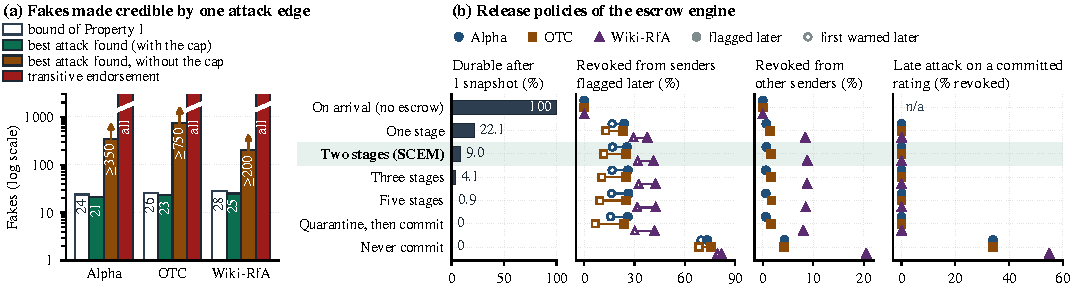
\includegraphics[width=\textwidth]{figures/fig_streams.pdf}
\caption{The credibility layer and escrow on the rating streams (no model training). (a)~Fake accounts that one attack edge makes credible. (b)~Seven release policies with credibility-weighted witnesses; the five that escrow and then commit share a mean delay of four snapshots. The four strips show the share of a rating that is durable one snapshot after arrival; the mass revoked from senders flagged later (at least two later warnings that outnumber the endorsements; hollow: first warned only after the rating); the mass revoked from other senders; and the share of a committed honest warning that five late fake witnesses revoke (unweighted witnesses, the attacker's best case).}
\label{fig:streams}
\end{figure*}

\begin{property}[First-layer invariance of retention, goal G3]
\label{prop:invariance}
Let account $v$ survive a set of deletions, let the tiers be fixed before the deletions, and let CPPR retain every deleted rating that $v$ received.
Then, in every snapshot, the gate weights of Eq.~\eqref{eq:cred_gate} over the ratings that $v$ receives equal their values before the deletions, and so does the first-layer aggregate of these ratings for fixed layer parameters and tier prototypes.
Moreover, a retained rating of a fake keeps the fake's tier weight: with $g$ attack edges, at most $\lfloor 2Kg \rfloor$ fakes carry more than $w_0$.
\end{property}
\begin{IEEEproof}
Eq.~\eqref{eq:cp_vpe} replaces each deleted rating by a rating from $P^{(t_k)}_{c(u_k)}$ to $v$ with the same sign in the same snapshot, and the pool node carries the weight $w_{c(u_k)}$ and the prototype of the rater's tier.
The multiset of pairs (tier weight, sign) over $\mathcal{E}^{(t)}_{\mathrm{in}}(v)$ and its size are therefore unchanged, and both the gate weights and the first-layer aggregate are functions of that multiset alone.
The second claim follows from Property~\ref{prop:btp}.
\end{IEEEproof}

Deleting honest warnings thus no longer removes them from what the model reads about the target.
The property stops at the first layer: deeper layers can differ, because a pool node has no incoming ratings. The property also holds the layer parameters and prototypes fixed, whereas the model is retrained on the retained graph with recomputed prototypes.
Section~\ref{subsec:results_vpe} measures the gain that remains.

\smallskip\noindent\textbf{Pseudonymity and Its Limit.}
By construction of Eq.~\eqref{eq:cp_vpe}, a retained rating no longer names its rater in the retained graph (goal G4). An insider who knows which raters share a pool, however, can still try to rank the true rater above the pool's other members.
CPPR therefore claims pseudonymity for use inside the controller, not anonymity (Section~\ref{subsec:results_vpe}).

\begin{table*}[!t]
\caption{Implementation and experimental settings. Triples list Bitcoin-Alpha, Bitcoin-OTC and Wiki-RfA.}
\label{tab:settings}
\centering
\footnotesize
\setlength{\tabcolsep}{4pt}
\begin{tabular}[t]{@{}>{\raggedright\arraybackslash}p{0.083\textwidth}>{\raggedright\arraybackslash}p{0.396\textwidth}@{}}
\toprule
\multicolumn{2}{@{}l}{\textbf{Data and backbone}} \\[1pt]
Ratings & Sign only; rating $0$ and self-loops dropped \\
Snapshots & $22$ in time order, of nearly equal size; a cut inside equal timestamps moves to their end; on Epinions-Dated, the $68.8\%$ at the crawl timestamp form the first \\
Retraining & Erased stream re-cut by the same rule; held-out snapshot kept \\
Features & Gaussian, diffused once on the normalized training adjacency \\
Layers & Three signed, widths $32$, $64$, $32$ (all $32$ on Epinions-Dated); linear map and ReLU \\
S3R & Position embedding; one causal sparse attention layer, $16$ heads ($8$ on Epinions-Dated), over $21$ snapshots; scores biased by a selective state-space block (state size $4$) \\
Head & Linear, $128$ parameters \\
Training & $150$ full-batch Adam steps, class-weighted cross-entropy; learning rate $0.005$, weight decay $10^{-5}$, gradient-norm clip $5$ \\
Test MCC & Distrust at $p_{uv} < 0.5$; held-out ratings between training accounts \\
\midrule
\multicolumn{2}{@{}l}{\textbf{Unlearning operators}} \\[1pt]
$\mathcal{U}_3$ & $10$ Adam steps: descend the retained loss, ascend that of $F$, mixed $0.99$ to $0.01$ \\
$\mathcal{U}_4$ & One damped Newton step, conjugate gradient with exact Hessian-vector products; damping $3.0$, $0.1$, $3.0$; not on Epinions-Dated (GPU memory) \\
$\mathcal{U}_5$ & One exact Newton step on the head \\
Selection & Seed $0$, $5$ cohort accounts ($3$ on Epinions-Dated): forget-set loss closest to retraining at a test-MCC drop of at most $0.02$ \\
\midrule
\multicolumn{2}{@{}l}{\textbf{Laundering study}} \\[1pt]
Targets & $50$ per network; $25$ with an endorsement, or all such accounts \\
Seeds & $0$ to $4$; $5$ to $9$ for the self-term check and the cautious prior \\
SGCN & PyTorch Geometric; two layers of width $64$ on $64$ spectral features; $200$ epochs \\
EigenTrust & Uniform pre-trust; teleport probability $0.15$ \\
Filters & Membership, declared role; rate: at most three requested ratings per target; fingerprint: head gradient in the $0.5\%$ to $99.5\%$ quantiles; direction: cosine with a one-step influence estimate at least the $1$st percentile of $30$ benign requests \\
Federated & $12$ warm-up rounds of $2$ local steps \\
\bottomrule
\end{tabular}\hfill
\begin{tabular}[t]{@{}>{\raggedright\arraybackslash}p{0.083\textwidth}>{\raggedright\arraybackslash}p{0.396\textwidth}@{}}
\toprule
\multicolumn{2}{@{}l}{\textbf{KEEPER}} \\[1pt]
BTP & Seeds from snapshots $0$ to $4$; $K = 12, 13, 14$; $\varepsilon = 0.02, 0.01, 0.50$; $q_{\mathrm{cap}} = 2\,q_{\min}$ \\
Engine & $N = 2$, $\phi = 0.5$, $A = 13.28$, $\lambda_{\max} = 2$ \\
Witnesses & Evidence of one witness about one account capped at $1$; reliability floors $0.35$ in the seed snapshots and $0.2$ afterwards for witnesses above Tier~$0$ \\
Module & Dimension $32$; learned $\phi \in [0.125, 0.5]$, $A = 53.1$; payload norm at most $5$; two-layer perceptron readout; an auxiliary loss of weight $0.05$ ties the hazard to the surprise of a rating \\
\midrule
\multicolumn{2}{@{}l}{\textbf{Retention and attack runs}} \\[1pt]
Targets & Per seed, $15$ lose all warnings and $5$ lose their warners' accounts; no two share a warner \\
Background & Single-rating requests on $2\%$ of the training ratings, none at a target; control arm: background only \\
Tiers & Frozen honest calibration; tiers recomputed with the fakes, under that calibration, in the inject-then-erase arms; a pool edge keeps the snapshot of the rating it replaces \\
A4 & A ring or star of $s = 3$ or $50$ fakes rates one target in one snapshot from $5$ to $20$ and deletes its accounts; bad-mouth victims hold at least three endorsements and no warning \\
A3 & $k \in \{1, 5, 10, 50\}$ fakes, $g \in \{0, 1, 2\}$ attack edges per attacked warning \\
Linkage & Candidates: the raters of a pool; pools with fewer than $10$ raters merged across snapshots of the same tier \\
Linkers & Hand-built: mean rank of structural similarity to the target, timing and the model's probability of the sign. Learned: histogram gradient boosting on these signals plus degree, activity, tier and pool size, trained on the other seeds \\
\midrule
\multicolumn{2}{@{}l}{\textbf{Statistics}} \\[1pt]
Estimates & Mean of per-seed means; $10{,}000$ bootstrap replicates over seeds and targets; Holm's correction at $5\%$ \\
Seeds & KEEPER: $5$ to $14$ for retention without attack edges and the end-to-end escrow test, $5$ to $9$ otherwise \\
\bottomrule
\end{tabular}
\end{table*}

\section{Experimental Evaluation}
\label{sec:results}

The evaluation asks what each mechanism buys and what it costs (RQ1 to RQ3) and how the three parts behave as one system (RQ4).

\subsection{Setup}
\label{subsec:datasets}

\noindent\textbf{Registered Protocol.}
Before running the experiments on KEEPER, we fixed the hypotheses, the endpoints, the decision rules and the random seeds in a protocol and committed it to our development repository (commit \texttt{150d85c}), without a third-party deposit. The released repository is a snapshot of the development repository and contains the protocol.
The seeds, $5$ to $14$, had been used by no earlier run, and every later clarification is logged next to the protocol.
The protocol registers eight statistical hypotheses and three exact checks, which need no statistical test. Table~\ref{tab:hypotheses} maps all eleven tests to the adversaries and to the properties of Section~\ref{sec:keeper} and gives the key result of each.
The $p$-value of a criterion is the larger of the $p$-values of a seed-level $t$-test and a bootstrap test.
A statistical hypothesis is confirmed only if every criterion is met on every network and its largest $p$-value survives Holm's correction over the eight hypotheses at $5\%$.
RQ1 to RQ3 report the registered tests, and RQ4 is descriptive.
Three results in RQ1 to RQ3 lie outside the registered tests and are marked as exploratory: the admission probes of RQ1, the component ablation of the engine in RQ2 and the gate normalization in RQ3.

\smallskip\noindent\textbf{Measures.}
A target's \emph{gain} is the change of its reputation (Eq.~\eqref{eq:gain}) in the attacker's direction.
A defense's \emph{cut} is one minus its mean gain divided by the mean gain without the defense.
In the retention experiments, a \emph{control-adjusted} gain subtracts the gain of the same target in a control run with the same unrelated background deletions but no attack.
Utility is the MCC of distrust prediction on the held-out snapshot.
Estimates are means over seeds. Each $95\%$ interval is the union of two intervals: a bootstrap interval that resamples seeds and targets, and a $t$-interval over seeds.
A threshold is \emph{met} when the interval's lower bound reaches it and \emph{inconclusive} when only the upper bound does. A hypothesis with a criterion that is not met is reported as \emph{not supported}; H7, whose intervals lie wholly above its criterion of $0.60$, is reported as \emph{contradicted}.

\smallskip\noindent\textbf{Implementation.}
Table~\ref{tab:settings} lists the settings that complete Sections~\ref{sec:system} to~\ref{sec:keeper}.
Every model trains in deterministic mode, each result file records its code version and the digest of the protocol, and the numbers of Sections~\ref{sec:laundering} and~\ref{sec:results} are generated from the released result files.

\smallskip\noindent\textbf{Deviations.}
Every change after registration is logged, and three matter for reading the results.
H5 is tested with one attacked warning per stream, because in a batch the attacks on other warners, the authors of warnings, reach a record through indirect paths; we report the differences in batched streams as descriptive.
The protocol assumed that a witness attack leaves the tiers of honest accounts unchanged, which holds only without attack edges; we count the accounts that move.
The withdrawal-count baseline of RQ3 has two more input features than the model that supplies the target's reputation before deletion, a confound that the log states.
The other entries change no endpoint; four of them are worth stating.
The protocol was committed when the first confirmatory job started.
With $50$ fake witnesses, an attacked stream holds one, two and four attacked warnings on the three networks, not one as registered.
H6a tests revocation within open escrow, because the module's records do not commit within the training horizon.
RQ4 comprises $120$ runs instead of the $18$ planned.

\subsection{RQ1: What Can Fake Accounts Buy From the Credibility Layer?}
\label{subsec:results_btp}

We evaluate the credibility layer directly on the three fully dated graphs; except for check H3a, no model is trained.

\smallskip\noindent\textbf{The Bound Is Nearly Tight, and the Cap Makes It Small.}
To see how close an attacker can come to the bound of Property~\ref{prop:btp}, an exploratory probe takes the five honest accounts whose single endorsement can carry the most trust.
Each of them endorses the hub of a star of fakes, in which the hub endorses all other fakes, and the star grows until no further fake is admitted.
The best attack that we found stays three fakes below the bound on every network (Fig.~\ref{fig:streams}a).
Without the cap, the strongest single endorsement admits at least $350$, $750$ and $200$ fakes; these are lower bounds, because the largest star that we probed was admitted whole.
Transitive endorsement admits every fake and BTP without the cap admits hundreds or more, so the cap is what turns one honest mistake from an open door into a bounded leak.
The bound also held in every trained run (check H3a): in the $150$ runs with BTP, none of $2{,}700$ groups of fakes had more credible members than the bound allows. What the admitted fakes achieve is tested in RQ3 (H3b).

\smallskip\noindent\textbf{Comparison With SybilRank.}
A second exploratory probe, run after the registered analysis, replaces BTP with SybilRank~\cite{cao2012aiding}. SybilRank runs on the endorsement graph without edge directions, with the seeds ($6\%$ to $33\%$ of the active accounts) and the $K$ steps of BTP.
SybilRank's threshold on degree-normalized trust is fixed on honest data at the largest value at which SybilRank keeps the same share of the accounts that transitive endorsement deems credible as BTP does; eligibility is as in Algorithm~\ref{alg:btp}.
One attack edge leads into a star or a ring of fakes; it comes from one of the five endorsers above or from one of the five accounts whose edge carries the most SybilRank trust.
The best attack that we found against SybilRank admits $23$, $31$ and $23$ fakes, against $21$, $23$ and $25$ for BTP.
With the threshold that keeps $90\%$, the registered share, SybilRank admits $22$, $29$ and $22$.
Neither method admits fewer fakes on all three networks; the two differ in what stands behind the number.
BTP's count is bounded for every region of fakes by Property~\ref{prop:btp}, whereas SybilRank exceeds that bound on Bitcoin-OTC ($31$ against $26$).
SybilRank's count is only the best attack that we found, and its guarantee assumes that random walks mix fast among honest accounts.
SybilRank also ignores the direction of an endorsement, so a fake that endorses an honest account creates the same edge as an attack edge, whereas BTP passes trust only from the endorser to the endorsed account.
The probe grants the attacker no such edge, so its counts favor SybilRank.

\smallskip\noindent\textbf{Honest Accounts Pay Little, Except Where Few Are Rated.}
BTP keeps $92.1\%$ to $94.5\%$ of the accounts that transitive endorsement deems credible.
On the Bitcoin networks, $14.5\%$ and $19.5\%$ of the accounts are in Tier~$0$.
On Wiki-RfA the share is $83.8\%$ ($84.3\%$ under transitive endorsement), because most accounts there are voters who are never rated themselves.
Their evidence counts with weight $w_0$ although it is honest, a limit that returns in RQ3.

\smallskip\noindent\textbf{Credibility Cannot Be Removed for Free.}
We let fresh fake accounts without any attack edge warn about $100$ honest victims of Tier~$2$ or~$3$.
When every rater's warnings count toward eligibility, five fakes per victim demote $69\%$ and $68\%$ of the victims on the Bitcoin networks, and $6\%$ on Wiki-RfA.
When only trusted raters' warnings count, as in KEEPER, the fakes demote none, the case $g = 0$ of Property~\ref{prop:btp}.

\subsection{RQ2: What Does Escrow Revoke, and Can It Be Abused?}
\label{subsec:results_scem}

The engine runs seven release policies on each training stream (Fig.~\ref{fig:streams}b).
Five of them escrow and then commit at the same mean delay of four snapshots: release through $N = 1$, $2$, $3$ or $5$ stages, with the commitment ages $18.42$, $13.28$, $11.21$ and $9.28$; and a quarantine that releases nothing and commits the surviving mass at age $4$.
The other two are commitment on arrival and a memory that never commits.
A sender is \emph{flagged later} if it receives at least two warnings after its rating, and more warnings than endorsements; it is \emph{first warned later} if it also had no warning when it rated, the stream's counterpart of the silent sender A2.

\smallskip\noindent\textbf{Escrow Is a Partial Defense.}
SCEM revokes $24.7\%$ to $41.3\%$ of the mass of ratings whose senders are flagged later, and $11.5\%$ to $31.9\%$ if the sender is first warned later.
It thus removes between a tenth and two fifths of what a sender who turns out to be distrusted contributed, at a cost of $0.7\%$ to $8.8\%$ of the mass of other senders.
On every stream the mass identity of Lemma~\ref{lem:mass} holds to within $6.7 \times 10^{-16}$.
All committing policies revoke similar shares.
More stages revoke slightly more from later-flagged senders, as Section~\ref{sec:scem} derives, but the increase flattens after two stages. For senders first warned later, more stages even revoke less on Bitcoin-OTC, because a sharply timed release leaves no mass in escrow when a late warning arrives.
The choice of two stages therefore rests on Property~\ref{prop:arrival}: two stages are the smallest number of stages with a flat start, which leaves $9.0\%$ of a rating durable after one snapshot instead of $22.1\%$.

\smallskip\noindent\textbf{Witness Evidence Drives Revocation.}
Revocation depends on what other accounts report about the sender.
In exploratory engine runs with unweighted witnesses, SCEM revokes $20.9\%$, $22.7\%$ and $49.8\%$ of the mass of later-flagged senders; the unweighted witnesses explain why these shares differ from those of Fig.~\ref{fig:streams}b.
With the witness evidence removed, so that only the self-surprise term feeds the hazard, the shares fall to $8.1\%$, $8.0\%$ and $10.1\%$, whereas removing the self-surprise term or supersession changes them by at most two percentage points.

\smallskip\noindent\textbf{Commitment Closes the Attack Window.}
A memory that never commits revokes the most, $73.4\%$ to $81.9\%$ of the mass of later-flagged senders, but it also revokes $4.2\%$ to $20.5\%$ of everyone else's and leaves every rating open to attack forever.
To test the time bound of Property~\ref{prop:window} (check H5), we attacked honest warnings one at a time with five unweighted fake witnesses, the attacker's best case. The fakes' warnings take effect only after the commitment age of the honest warning.
Under every committing policy, the committed rating was unchanged in every case, with a difference of exactly zero; for SCEM's policy, these are $958$ cases at the two snapshot lengths studied below. In the memory that never commits, the same late attacks revoke a third to more than half of the honest warning.
The check attacks one warning per stream. When many raters are attacked in one stream, an attack on another rater can still reach a rating in escrow through the reliability of other accounts and the self-surprise term, by at most $1.6 \times 10^{-4}$ for SCEM's policy.
The price of commitment is calendar time: $13.28$ snapshots are between $1{,}147$ and $2{,}005$ days at our snapshot length.
Cutting the full streams into four times as many snapshots reduces the commitment age in days to a quarter. The shares revoked from later-flagged senders then become $24.8\%$, $30.7\%$ and $30.5\%$, against $25.1\%$, $24.3\%$ and $36.9\%$ at the original length. These full streams include the held-out snapshot, hence the small differences from Fig.~\ref{fig:streams}b.

\begin{figure}[!t]
\centering
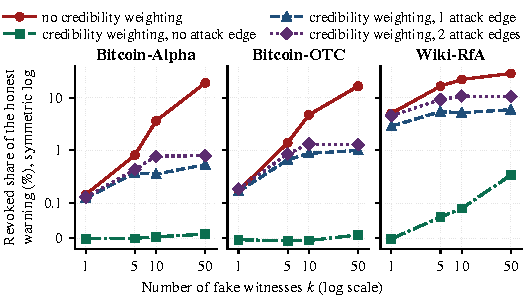
\includegraphics[width=\columnwidth]{figures/fig_witness.pdf}
\caption{Fake-witness attack on escrow: $k$ fakes warn about an honest rater one snapshot after its warning, to revoke that warning in escrow. Each panel shows the mean revoked share of the honest warning, attacked minus clean stream; the vertical axis is linear below $0.1\%$ and logarithmic above.}
\label{fig:witness}
\end{figure}

\smallskip\noindent\textbf{Credibility Weighting Against Fake Witnesses.}
Adversary A3 attacks the honest warners of the laundering cohort: $k$ fresh fake accounts, linked by a directed ring of endorsements, warn about a warner one snapshot after its warning, while that warning is in escrow (Fig.~\ref{fig:witness}).
Their $g$ attack edges come from honest accounts of Tier~$2$ or~$3$, and the fakes of one attacked stream stay below $2\%$ of the active accounts.
Without credibility weighting the attack scales with the number of fakes: $50$ fakes revoke up to $28.8\%$ of the honest warning on average, and up to $64.6\%$ of a single one.
With credibility weighting, fresh fakes without attack edges revoke almost nothing: for $50$ fakes the mean is at most $0.011\%$ on the Bitcoin networks and $0.34\%$ on Wiki-RfA, which meets the registered criterion of at most $1\%$ on every network (check H4).
Fakes that first build reliability by rating one another from the earliest snapshot an attacker may use, a variant outside the registered check, revoke $0.10\%$, $0.14\%$ and $2.6\%$ on average.
With attack edges the effect is bounded per edge, as Property~\ref{prop:window} states, and no longer grows with the number of fakes: with one attack edge, $5$ to $50$ fakes revoke on average at most $1.0\%$ on the Bitcoin networks and $5.2\%$ to $5.9\%$ on Wiki-RfA.
Single warnings can lose more than the mean: with two attack edges the $95$th percentile reaches $6\%$ on the Bitcoin networks and $42\%$ on Wiki-RfA.
Each attack edge also moves between $1$ and $39$ honest accounts across a tier boundary, because the admitted fakes shift the terciles.

\smallskip\noindent\textbf{End to End, No Measurable Effect on Predictions.}
The engine results concern escrow weights.
To test predictions, we let three fresh silent senders rate a target, $+1$ to whitewash a distrusted target or $-1$ to bad-mouth a well-reputed one, and two witnesses of Tier~$2$ or~$3$ warn about each sender one snapshot later.
Each seed attacks $15$ targets of each kind, and we train the backbone with and without escrow on ten seeds.
Neither of the two registered hypotheses, H6a and H6b, is confirmed (Table~\ref{tab:hypotheses}).
Relative to SCEM without its hazard (H6a), every interval of the reduction of the senders' effect includes zero.
Relative to the backbone without escrow (H6b), the interval lies above zero only for whitewashing on Wiki-RfA ($+0.094$, interval $0.009$ to $0.180$).
Two facts about the module bear on this result.
First, the module's commitment age of $53.1$ snapshots lies beyond the training horizon (the learned rate is about $0.31$). Second, a rating also reaches the target's representation through the snapshot embedding, which escrow does not govern.
LocalGDTE-SCEM matches the backbone's test MCC on the Bitcoin networks ($0.362$ and $0.340$ against $0.352$ and $0.329$) and loses on Wiki-RfA ($0.170$ against $0.223$).

\subsection{RQ3: Does Retention Remove Laundering and Confine Fake Accounts?}
\label{subsec:results_vpe}

The retention runs use the gated model of Section~\ref{sec:cppr} on the escrow module in sequence mode, with one record per account and snapshot instead of one per rating (Section~\ref{sec:scem}). They draw their targets from the cohort without stratification (Table~\ref{tab:settings}).
In the \emph{direct} arm, raters delete their warnings; in the \emph{whitewash} and \emph{bad-mouth} arms, fakes rate a target and delete their accounts; a \emph{control} arm carries only the unrelated background deletions that every arm shares.
Gains in this section are therefore not comparable with those of Section~\ref{sec:laundering}.

\begin{table}[!t]
\caption{Retention methods: mean reputation gain of the target (positive values favor the attacker) on Bitcoin-Alpha (A), Bitcoin-OTC (O) and Wiki-RfA (W). Direct: raters delete up to three authentic warnings. Whitewash: three fakes without attack edges rate the target $+1$, then delete themselves.}
\label{tab:cppr_main}
\centering
\footnotesize
\setlength{\tabcolsep}{2.4pt}
\begin{tabular}{@{}>{\raggedright\arraybackslash}p{0.72in}rrrrrr@{}}
\toprule
 & \multicolumn{3}{c}{\textbf{Direct laundering}} & \multicolumn{3}{c}{\textbf{Whitewash}} \\
\cmidrule(lr){2-4}\cmidrule(l){5-7}
\textbf{Method} & A & O & W & A & O & W \\
\midrule
Plain erasure & $+0.175$ & $+0.154$ & $+0.238$ & \multicolumn{3}{c}{n/a} \\
Withdrawal counts & $+0.173$ & $+0.159$ & $+0.279$ & $+0.007$ & $+0.012$ & $+0.023$ \\
Per-rating pseudonym & $+0.083$ & $+0.046$ & $+0.129$ & $+0.008$ & $+0.007$ & $+0.034$ \\
Single pool & $-0.059$ & $-0.052$ & $-0.022$ & $+0.053$ & $+0.075$ & $+0.325$ \\
Retain with author & $0$ & $0$ & $0$ & $+0.023$ & $+0.011$ & $+0.024$ \\
\textbf{CPPR} & $\mathbf{-0.030}$ & $\mathbf{-0.038}$ & $\mathbf{+0.010}$ & $\mathbf{+0.044}$ & $\mathbf{+0.023}$ & $\mathbf{+0.011}$ \\
\bottomrule
\end{tabular}
\par\smallskip
\parbox{\columnwidth}{\footnotesize Seeds $5$ to $9$; gains not control-adjusted (adjusted: Fig.~\ref{fig:retention}). On the Bitcoin networks, gains below about $0.06$ are within retraining noise. Withdrawal counts: plain erasure plus the counts of withdrawn positive and negative ratings as two input features. Per-rating pseudonym: each deleted rating moves to its own new node at its rater's tier weight. Retain with author: the rating keeps its author in the model, so the direct gain is $0$ by construction. n/a: plain erasure removes the fakes' ratings.}
\end{table}

\begin{figure*}[!t]
\centering
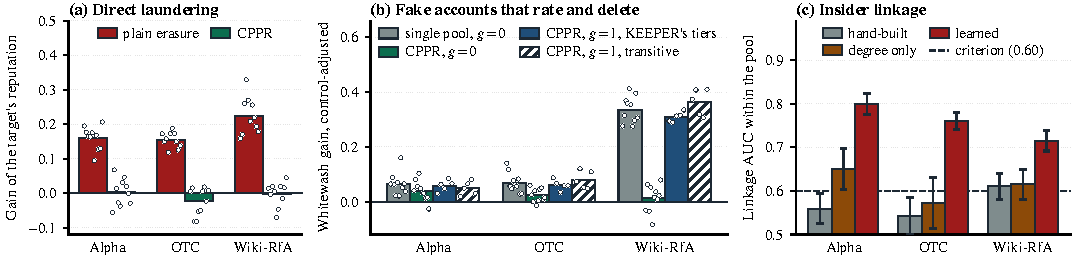
\includegraphics[width=\textwidth]{figures/fig_retention.pdf}
\caption{Retention on the confirmatory runs (bars: means over seeds; dots: seeds). (a)~Direct laundering on ten fresh seeds: reputation gain under plain erasure and control-adjusted gain under CPPR. (b)~Control-adjusted whitewash gain when fakes with $g$ attack edges rate a target $+1$ and delete themselves, under a single pool or under CPPR with BTP (KEEPER's) or transitive-endorsement tiers. (c)~Insider linkage: area under the ROC curve (AUC) for ranking a retained rating's true rater above the other pool members, with $95\%$ intervals; chance is $0.5$, and the dashed line is the registered criterion.}
\label{fig:retention}
\end{figure*}

\smallskip\noindent\textbf{Retention Cuts Direct Laundering by 98\% or More.}
On ten fresh seeds, plain erasure raises a target's reputation by more than CPPR does on every network (Fig.~\ref{fig:retention}a). The difference is $0.173$, $0.174$ and $0.225$ on Bitcoin-Alpha, Bitcoin-OTC and Wiki-RfA ($p \le 0.0001$ each).
Here the cut compares CPPR's control-adjusted gain with the gain of plain erasure, which has no control run. A cut above $100\%$ means that the target ends below its reputation before the deletions.
CPPR cuts the laundering gain by $98\%$ or more, and the lower interval bounds reach the registered threshold of $80\%$ on every network (Table~\ref{tab:hypotheses}).
The interval criteria of hypothesis H1 are thus met on all three networks.
The weakest criterion of H1, the threshold on Bitcoin-Alpha, has $p = 0.023$, which does not survive Holm's correction (adjusted $p = 0.19$), so we report H1 as met by its intervals but not confirmed.
Retention costs no accuracy relative to plain erasure: the test MCC differs by $-0.002$, $-0.001$ and $+0.002$, with intervals that include zero.

\smallskip\noindent\textbf{Why Pools, and Why One per Tier.}
Table~\ref{tab:cppr_main} compares CPPR with the obvious alternatives on seeds $5$ to $9$ without control adjustment, so its entries differ slightly from the ten-seed, control-adjusted values of Fig.~\ref{fig:retention}a.
Telling the model how many ratings were withdrawn from an account (withdrawal counts) does not help in the form that we tested: the gain stays at that of plain erasure.
Giving every deleted rating its own pseudonym leaves $47\%$, $30\%$ and $54\%$ of the gain, although this scheme meets the premise of Property~\ref{prop:invariance} as CPPR does.
First-layer invariance is therefore not sufficient. The difference must arise in the deeper layers, where a node that sends one rating and a pool node that sends many are represented differently; we did not isolate this effect.
A single pool per snapshot removes direct laundering as CPPR does but lets fake accounts whitewash a target, most clearly on Wiki-RfA.
Keeping the rating with its author removes laundering by construction, but it keeps the rater's identity in the model, which retention under data minimization must avoid.
The count normalization of the gate matters as well.
In exploratory runs on seeds $0$ to $4$ with transitive-endorsement tiers and without a control arm, dividing by the sum of the weights instead lowers CPPR's cut of the single-pool whitewash gain from $100.5\%$, $66.4\%$ and $88.5\%$ to $52.5\%$, $34.1\%$ and $14.8\%$.

\smallskip\noindent\textbf{Confinement of Fakes Without Attack Edges Is Not Supported as Registered.}
Hypotheses H2b and H2w require that, relative to a single pool, CPPR cuts the effect of inject-then-erase fakes by at least $80\%$ on every network. Neither is supported as registered (Table~\ref{tab:hypotheses}).
For bad-mouthing the criterion is met on the Bitcoin networks, with lower bounds of $91\%$ and $84\%$, and inconclusive on Wiki-RfA, where the lower bound is $79\%$.
For whitewashing the criterion is met on Wiki-RfA, where the single-pool gain is large (lower bound $85\%$).
On the Bitcoin networks the single-pool whitewash gain is small ($+0.064$ and $+0.070$ after control adjustment), so the cut has wide intervals and removal is not established there.

\smallskip\noindent\textbf{One Attack Edge Buys Few Fakes, and Few Suffice.}
The bound of Property~\ref{prop:btp} limits how many fakes one endorsement admits, not what the admitted fakes achieve.
The attacker chooses a ring or a star of $3$ or $50$ fakes and an endorser. The endorser is drawn at random from the honest accounts of Tier~$2$ or~$3$, or chosen as an account whose endorsement carries the most trust. Each seed then uses the choice that is best for the attacker on the other seeds.
Hypothesis H3b, that this best whitewash gain with one attack edge is smaller under BTP than under transitive endorsement, is not supported on any network: every interval of the difference includes zero (Fig.~\ref{fig:retention}b).
The attacker's best response is a group of three fakes endorsed by one of the most credible honest accounts, far below the bound of $24$ to $28$.
Three credible fakes raise the target by at most $0.07$ on the Bitcoin networks but by $0.32$ on Wiki-RfA.
We attribute the size of the latter to the Tier-$0$ share of Wiki-RfA: most of its honest ratings are discounted to $w_0$, so a few credible ratings dominate what the gate passes.
The cap binds only for large groups: of $50$ fakes, BTP admits a single one, and on Wiki-RfA the control-adjusted gain then falls from $0.37$ under transitive endorsement to $0.12$.
Retention does not measurably add to this gain, because with one attack edge CPPR's whitewash gain does not differ measurably from that of fakes who keep their ratings (differences $-0.004$, $-0.037$ and $+0.024$, intervals including zero; seeds $5$ to $9$, not control-adjusted).

\smallskip\noindent\textbf{The Gated Model Has a Price.}
Relative to the plain backbone of Section~\ref{subsec:prelim} (S3R, no gate), the test MCC of the gated model under CPPR changes by $+0.044$, $-0.012$ and $-0.092$ (direct arm, ten seeds).
The two models differ in the gate, the tier prototypes and the temporal encoder, which is the escrow module in the gated model, so the change is not the gate's alone.
Both can contribute on Wiki-RfA: most of its honest evidence is discounted to Tier~$0$ (RQ1), and the escrow module alone also loses accuracy there (RQ2).
We did not separate the two.

\smallskip\noindent\textbf{Retained Raters Remain Linkable.}
Pseudonymous retention does not hide a rater from an insider.
The insider ranks the members of a pool by how likely each is the true rater of a retained rating. We score the attempt by the area under the ROC curve (AUC) within the pool. For this measurement only, a pool with fewer than $10$ raters is merged with the same tier's pools of other snapshots.
A hand-built attacker that combines three signals (the candidate's structural similarity to the target, the timing of its remaining ratings and the model's prediction) reaches an AUC of $0.559$, $0.543$ and $0.611$.
A learned attacker, a gradient-boosting classifier that is trained on other seeds and also sees the candidate's degree, activity and tier, reaches $0.72$ to $0.80$. Every $95\%$ interval lies above our criterion of $0.60$, so hypothesis H7 is contradicted (Fig.~\ref{fig:retention}c).
The learned attacker's first guess is the true rater in $18.5\%$ to $22.7\%$ of the cases, about five times chance.
The learned attacker relies mostly on a rater's degree in the retained graph, which alone gives an AUC of $0.650$, $0.573$ and $0.615$. Deleting ratings leaves a footprint in what remains of the rater's activity, the structural re-identification known from anonymized social networks~\cite{narayanan2009deanonymizing}.
Retained ratings are linked about as well under per-rating pseudonyms ($0.795$, $0.745$ and $0.719$) and under tiers from transitive endorsement ($0.745$, $0.741$ and $0.714$).

\subsection{RQ4: KEEPER as One System}
\label{subsec:results_combined}

So far each mechanism ran on its own backbone.
We now train the escrow model of RQ2, which keeps one record per rating, with credibility-weighted witnesses and CPPR's gate. On seeds $5$ to $9$ we repeat three attacks: direct laundering, whitewashing by fakes without attack edges, and fake witnesses.
The protocol registers this experiment as descriptive, so we draw no superiority conclusion from it.

\smallskip\noindent\textbf{Retention Keeps Its Effect.}
Plain erasure raises a target's reputation by $0.198$, $0.252$ and $0.226$, whereas under CPPR the change is $-0.060$, $-0.051$ and $-0.037$.

\smallskip\noindent\textbf{The Confinement of Fakes Does Not Carry Over.}
Without attack edges, fakes whitewash a target by $0.044$, $0.098$ and $0.224$ under CPPR and by $0.091$, $0.118$ and $0.243$ under a single pool, although no fake is admitted above Tier~$0$. On the model of Table~\ref{tab:cppr_main}, CPPR had held the same attack on Wiki-RfA to $0.011$.
The cause is a path that the gate does not cover.
The gate weights the messages of the convolution layers (Eq.~\eqref{eq:cred_gate}), whereas the escrow memory adds the released part of every incoming rating to the receiver's durable memory with a mass that does not depend on the sender's tier.
The ratings of the Tier-$0$ pool therefore reach the target through escrow, a path outside Property~\ref{prop:invariance}.
Weighting each escrow record by its sender's tier weight would close the path; we have not evaluated this change.

\smallskip\noindent\textbf{Fake Witnesses Have No Measurable Effect.}
Five fakes per warning, with zero or one attack edge, warn about the honest warners of the direct targets.
The targets' reputations change by at most $0.019$ in the attacker's favor, with credibility weighting on or off, in line with the end-to-end result of RQ2.

\smallskip\noindent\textbf{Overhead.}
The credibility layer is a sparse propagation: computing the tiers of every account for all $21$ training snapshots, calibration included, takes less than half a second.
At the module's dimension of $32$, the state of the escrow memory peaks at $3.59$, $5.38$ and $20.56$~MiB on our streams.
CPPR adds at most four pool nodes per snapshot, one per tier.
We did not measure the training cost of the gated and escrow models separately; like exact erasure, every retention method is served by retraining.

\section{Discussion and Limitations}
\label{sec:discussion}

The results hold under legal and technical conditions that this section makes explicit.

\subsection{When May a Platform Retain a Deleted Rating?}
\label{subsec:gdpr}

SCEM and CPPR apply under different legal conditions, so we separate three regimes under GDPR Article~17~\cite{gdpr2016}.
The realistic deleter in all regimes is a rater who withdraws its own ratings. A request by the rated account to erase what others wrote is a weaker claim, because the exemption for freedom of expression and information in Art.~17(3)(a) can apply.
\emph{Regime~1, erasure without retention.}
When no basis for retention exists, the platform must erase the deleted ratings and serve a model that depends on the remaining graph alone.
By the indistinguishability argument of Section~\ref{sec:laundering}, laundering cannot be prevented in this regime. SCEM still governs how new ratings enter the memory, but it does not restore an erased warning.
\emph{Regime~2, pseudonymous retention inside the controller.}
Retention needs a lawful basis independent of the rater's consent, such as the controller's legitimate interest in fraud prevention under Art.~6(1)(f)~\cite{edpb2024legit} or the defense of legal claims under Art.~17(3)(e). The controller must also document the balancing of interests.
CPPR is built for this regime and follows data minimization: a fraud model needs a rating's verdict and its rater's credibility, but not the rater's identity.
The rater can still object under Art.~21(1); retention then continues only if the controller demonstrates compelling legitimate grounds that override the rater's interests.
The regime also needs three organizational controls that we do not evaluate: destroying the map from raters to pool nodes, restricting the pool nodes to fraud scoring, and bounding the retention period.
\emph{Regime~3, release outside the controller.}
Releasing the retained graph would need anonymity, which CPPR does not provide (Section~\ref{subsec:results_vpe}).

\subsection{Composing Escrow and Retention}
\label{subsec:composition}

A rating reaches the model along two paths, the snapshot embedding of the convolution layers and the escrow memory, and in our implementation each mechanism covers only its own path.
A silent sender's rating reaches its target through the snapshot embedding, which escrow does not govern, and the Tier-$0$ pool reaches its target through escrow, which the gate does not weight.
A composed defense must therefore apply the credibility weight and the escrow rule to both paths, a change that we leave to future work.
Coupling escrow and retention more tightly, by retaining only the mass that escrow has released, would leave a fake account that rates a target and deletes itself $x$ snapshots later at most $(\phi x)^2/2$ of a rating. Such coupling would also discard, however, the unreleased part of an honest warning deleted while young.

\subsection{Limitations}
\label{subsec:limitations}

Ten limitations bound the claims of this paper.
(1)~\emph{Model-derived outcome.} Reputation is the model's prediction, not an enforcement log.
(2)~\emph{One backbone.} The attack is shown on two GNNs; KEEPER is evaluated on LocalGDTE only, whose test MCC is modest ($0.22$ to $0.35$).
(3)~\emph{Assumptions of the credibility layer.} The layer needs honest seeds, accounts that are rated, and a calibration on a graph without the fakes, which a platform can only approximate. On Wiki-RfA, $84\%$ of the accounts stay in Tier~$0$, and the gated model loses $0.092$ in test MCC against the plain backbone.
(4)~\emph{Attack edges.} One honest endorsement makes up to $\lfloor 2K \rfloor$ fakes credible and moves some honest accounts across tier boundaries. The bound also does not limit what a few credible fakes achieve: three raise a target by $0.32$ on Wiki-RfA, and a single credible fake witness is about as effective as an unweighted one on the Bitcoin networks and about half as effective on Wiki-RfA (Fig.~\ref{fig:witness}).
(5)~\emph{Escrow is partial.} SCEM revokes between a tenth and two fifths of the mass of senders who turn out to be distrusted, its commitment age is long in calendar time, and its trained form did not measurably change predictions and lost accuracy on Wiki-RfA.
(6)~\emph{Retention.} On the Bitcoin networks, fake accounts without attack edges still whitewash a target under CPPR, and in the combined system they do so on every network. The gate divides by the number of ratings that a target receives in a snapshot, so a flood of Tier-$0$ ratings in the snapshot of honest warnings would dilute those warnings; we did not evaluate this attack. CPPR is served by retraining after each batch of deletions, and we did not test whether re-pointing the ratings without retraining suffices.
(7)~\emph{Linkage.} An insider links retained ratings to their raters, so CPPR must stay inside the controller.
(8)~\emph{Unconfirmed hypotheses.} None of the eight registered statistical hypotheses is confirmed under our rule (Table~\ref{tab:hypotheses}).
(9)~\emph{Separate settings.} The laundering and the retention results use different models, target samples and background deletions, so their gains are not comparable.
(10)~\emph{Mistaken warnings.} We take every warning as authentic evidence. Under retention, erasing a warning no longer withdraws its verdict, so a platform that retains must give raters another way to correct a warning.

\subsection{Ethical Considerations}
\label{subsec:ethics}

All experiments run on public research datasets; no live platform was probed, and no user was contacted.
The attack uses only erasure requests that any rater can already make, and we describe it together with a defense and with the measured limits of that defense.

\section{Conclusion}
\label{sec:conclusion}

Erasing a few authentic warnings launders the reputation of a distrusted account. The effect comes from the graph that the model reads, so better unlearning cannot remove it; the request and parameter filters that we tested did not remove it either.
KEEPER governs the evidence instead, with a credibility layer that admits a bounded number of fakes per honest endorsement.
Before a rating becomes permanent, escrow lets credible warnings about its sender revoke part of it, and commitment bounds the time in which fake witnesses can interfere.
At deletion, where the law allows retention, a pool pseudonym for the deleted raters of one snapshot and credibility tier keeps the warning in what the model reads. Retention cuts the laundering gain by $98\%$ or more on three networks, an effect that our multiplicity correction does not confirm.
Open problems remain. Escrow's trained form did not measurably change predictions in our end-to-end test; the credibility layer bounds how many fakes one endorsement makes credible, but not what a few of them achieve; a composed system must gate the escrow path as well; the gated model loses accuracy where few accounts are rated; and an insider can still link retained raters.

\begin{thebibliography}{99}
\providecommand{\url}[1]{#1}
\providecommand{\newblock}{\relax}
\providecommand{\bibinfo}[2]{#2}

\bibitem{kumar2016edge}
S.~Kumar, F.~Spezzano, V.~S. Subrahmanian, and C.~Faloutsos, ``Edge weight
  prediction in weighted signed networks,'' in \emph{Proc. IEEE
  Int. Conf. on Data Mining (ICDM)}, 2016, pp. 221--230.

\bibitem{kumar2018rev2}
S.~Kumar, B.~Hooi, D.~Makhija, M.~Kumar, C.~Faloutsos, and V.~S. Subrahmanian,
  ``{REV2}: Fraudulent user prediction in rating platforms,'' in
  \emph{Proc. ACM Int. Conf. on Web Search and Data
  Mining (WSDM)}, 2018, pp. 333--341.

\bibitem{west2014exploiting}
R.~West, H.~S. Paskov, J.~Leskovec, and C.~Potts, ``Exploiting social network
  structure for person-to-person sentiment analysis,'' \emph{Transactions of
  the Association for Computational Linguistics (TACL)}, vol.~2, pp. 297--310,
  2014.

\bibitem{derr2018signed}
T.~Derr, Y.~Ma, and J.~Tang, ``Signed graph convolutional networks,'' in
  \emph{Proc. IEEE Int. Conf. on Data Mining
  (ICDM)}, 2018, pp. 929--934.

\bibitem{rossi2020temporal}
E.~Rossi, B.~Chamberlain, F.~Frasca, D.~Eynard, F.~Monti, and M.~Bronstein,
  ``Temporal graph networks for deep learning on dynamic graphs,'' in
  \emph{ICML Workshop on Graph Representation Learning and Beyond}, 2020,
  arXiv:2006.10637.

\bibitem{gdpr2016}
{European Parliament and Council of the European Union}, ``Regulation ({EU})
  2016/679 (General Data Protection Regulation),'' \emph{Official Journal of
  the European Union}, vol. L119, pp. 1--88, 2016.

\bibitem{cao2015towards}
Y.~Cao and J.~Yang, ``Towards making systems forget with machine unlearning,''
  in \emph{Proc. IEEE Symp. on Security and Privacy (S\&P)},
  2015, pp. 463--480.

\bibitem{bourtoule2021machine}
L.~Bourtoule, V.~Chandrasekaran, C.~A. Choquette-Choo, H.~Jia, A.~Travers,
  B.~Zhang, D.~Lie, and N.~Papernot, ``Machine unlearning,'' in
  \emph{Proc. IEEE Symp. on Security and Privacy (S\&P)},
  2021, pp. 141--159.

\bibitem{chen2022graph}
M.~Chen, Z.~Zhang, T.~Wang, M.~Backes, M.~Humbert, and Y.~Zhang, ``Graph
  unlearning,'' in \emph{Proc. ACM SIGSAC Conf. on Computer
  and Communications Security (CCS)}, 2022, pp. 499--513.

\bibitem{ye2014strategic}
S.~Ye, G.~Gao, and S.~Viswanathan, ``Strategic behavior in online reputation systems: Evidence from revoking on {eBay},'' \emph{MIS Quart.}, vol.~38, no.~4, pp. 1033--1056, 2014.

\bibitem{di2023hidden}
J.~Z. Di, J.~Douglas, J.~Acharya, G.~Kamath, and A.~Sekhari, ``Hidden poison:
  Machine unlearning enables camouflaged poisoning attacks,'' in \emph{Advances in
  Neural Information Processing Systems (NeurIPS)}, vol.~36, 2023.

\bibitem{zhang2026attack}
J.~Zhang, Y.~Wang, and S.~Wang, ``Attack by unlearning: Unlearning-induced adversarial attacks on graph neural networks,'' arXiv:2603.18570, 2026.

\bibitem{zugner2018adversarial}
D.~Z{\"u}gner, A.~Akbarnejad, and S.~G{\"u}nnemann, ``Adversarial attacks on neural networks for graph data,'' in \emph{Proc. ACM SIGKDD Int. Conf. Knowl. Discovery Data Mining (KDD)}, 2018, pp. 2847--2856.

\bibitem{zhao2023static}
C.~Zhao, W.~Qian, R.~Ying, and M.~Huai, ``Static and sequential malicious attacks in the context of selective forgetting,'' in \emph{Proc. Adv. Neural Inf. Process. Syst. (NeurIPS)}, vol.~36, 2023.

\bibitem{qian2023towards}
W.~Qian, C.~Zhao, W.~Le, M.~Ma, and M.~Huai, ``Towards understanding and
  enhancing robustness of deep learning models against malicious unlearning
  attacks,'' in \emph{Proc. ACM SIGKDD Conf. on Knowledge
  Discovery and Data Mining (KDD)}, 2023, pp. 1932--1942.

\bibitem{wu2023gif}
J.~Wu, Y.~Yang, Y.~Qian, Y.~Sui, X.~Wang, and X.~He, ``{GIF}: A general graph
  unlearning strategy via influence function,'' in \emph{Proc. ACM
  Web Conf. (WWW)}, 2023, pp. 651--661.

\bibitem{kurmanji2024towards}
M.~Kurmanji, P.~Triantafillou, J.~Hayes, and E.~Triantafillou, ``Towards
  unbounded machine unlearning,'' in \emph{Advances in Neural Information
  Processing Systems (NeurIPS)}, vol.~36, 2023.

\bibitem{tan2024unlink}
J.~Tan, F.~Sun, R.~Qiu, D.~Su, and H.~Shen, ``Unlink to unlearn: Simplifying edge unlearning in {GNNs},'' in \emph{Companion Proc. ACM Web Conf. (WWW)}, 2024.

\bibitem{hu2024duty}
H.~Hu, S.~Wang, J.~Chang, H.~Zhong, R.~Sun, S.~Hao, H.~Zhu, and M.~Xue, ``A
  duty to forget, a right to be assured? Exposing vulnerabilities in machine
  unlearning services,'' in \emph{Proc. Network and Distributed
  System Security Symp. (NDSS)}, 2024.

\bibitem{unlearnguard2025}
W.~Wang, Q.~Ma, Z.~Zhang, Y.~Liu, Z.~Liu, and M.~Fang, ``Poisoning attacks and
  defenses to federated unlearning,'' in \emph{Companion Proc. ACM
  Web Conf. (WWW Companion)}, 2025, pp. 1365--1369.

\bibitem{blanchard2017machine}
P.~Blanchard, E.~M. El~Mhamdi, R.~Guerraoui, and J.~Stainer, ``Machine learning
  with adversaries: Byzantine tolerant gradient descent,'' in \emph{Advances in
  Neural Information Processing Systems (NeurIPS)}, vol.~30, 2017, pp.
  119--129.

\bibitem{yin2018byzantine}
D.~Yin, Y.~Chen, R.~Kannan, and P.~Bartlett, ``Byzantine-robust distributed
  learning: Towards optimal statistical rates,'' in \emph{Proc. Int. Conf. on Machine Learning (ICML)}, 2018, pp. 5650--5659.

\bibitem{kamvar2003eigentrust}
S.~D. Kamvar, M.~T. Schlosser, and H.~Garcia-Molina, ``The {EigenTrust}
  algorithm for reputation management in {P2P} networks,'' in \emph{Proc.
  Int. World Wide Web Conf. (WWW)}, 2003, pp. 640--651.

\bibitem{friedman2001social}
E.~J. Friedman and P.~Resnick, ``The social cost of cheap pseudonyms,'' \emph{J. Econ. Manage. Strategy}, vol.~10, no.~2, pp. 173--199, 2001.

\bibitem{cheng2005sybilproof}
A.~Cheng and E.~Friedman, ``Sybilproof reputation mechanisms,'' in \emph{Proc. ACM SIGCOMM Workshop Econ. Peer-to-Peer Syst. (P2PECON)}, 2005, pp. 128--132.

\bibitem{gyongyi2004combating}
Z.~Gy{\"o}ngyi, H.~Garcia-Molina, and J.~Pedersen, ``Combating web spam with {TrustRank},'' in \emph{Proc. Int. Conf. Very Large Data Bases (VLDB)}, 2004, pp. 576--587.

\bibitem{yu2006sybilguard}
H.~Yu, M.~Kaminsky, P.~B. Gibbons, and A.~Flaxman, ``{SybilGuard}: Defending
  against {Sybil} attacks via social networks,'' in \emph{Proc. ACM SIGCOMM Conf.}, 2006, pp. 267--278.

\bibitem{cao2012aiding}
Q.~Cao, M.~Sirivianos, X.~Yang, and T.~Pregueiro, ``Aiding the detection of
  fake accounts in large scale social online services,'' in \emph{Proc.
  USENIX Symp. on Networked Systems Design and Implementation
  (NSDI)}, 2012, pp. 197--210.

\bibitem{tran2009sybil}
D.~N. Tran, B.~Min, J.~Li, and L.~Subramanian, ``Sybil-resilient online content
  voting,'' in \emph{Proc. USENIX Symp. on Networked Systems
  Design and Implementation (NSDI)}, 2009, pp. 15--28.

\bibitem{devries1990gamma}
B.~de~Vries and J.~C. Principe, ``The gamma model---a new neural model for
  temporal processing,'' \emph{Neural Networks}, vol.~5, no.~4, pp. 565--576,
  1992.

\bibitem{hurtado2019generalized}
P.~J. Hurtado and A.~S. Kirosingh, ``Generalizations of the linear chain
  trick: Incorporating more flexible dwell time distributions into mean field
  {ODE} models,'' \emph{Journal of Mathematical Biology}, vol.~79, no.~5, pp.
  1831--1883, 2019.

\bibitem{edpb2025pseudo}
European Data Protection Board, ``Guidelines 01/2025 on pseudonymisation,'' Version 1.0 (adopted for public consultation), Jan. 2025.

\bibitem{narayanan2009deanonymizing}
A.~Narayanan and V.~Shmatikov, ``De-anonymizing social networks,'' in \emph{Proc. IEEE Symp. Security and Privacy (S\&P)}, 2009, pp. 173--187.

\bibitem{gu2023mamba}
A.~Gu and T.~Dao, ``{Mamba}: Linear-time sequence modeling with selective state
  spaces,'' in \emph{Conf. on Language Modeling (COLM)}, 2024,
  arXiv:2312.00752.

\bibitem{massa2005controversial}
P.~Massa and P.~Avesani, ``Controversial users demand local trust metrics: An
  experimental study on {Epinions.com} community,'' in \emph{Proc. Nat. Conf. on Artificial Intelligence (AAAI)}, 2005, pp. 121--126.

\bibitem{edpb2024legit}
{European Data Protection Board (EDPB)}, ``Guidelines 1/2024 on processing of
  personal data based on Article 6(1)(f) {GDPR},'' 2024.

\end{thebibliography}
\end{document}
